\documentclass[a4paper, 12pt]{article}
\usepackage[fontsize=12pt]{scrextend}

% ABNT - PACOTE DE ACENTUAÇÃO
\usepackage[utf8]{inputenc} 

% MARGENS LEFT RIGHT TOP E BOTTOM
\usepackage[lmargin=2cm,
            tmargin=0.6cm,
            rmargin=2cm,
            bmargin=3cm,
            headsep=0.0cm,
            includeheadfoot]{geometry}

\setlength\headheight{2.8cm}

% LEVA O ESTILO DO TEXTO PARA OUTROS PROGRAMAS TIPO WORD
\usepackage[T1]{fontenc}

% PÕE O PRIMEIRO PARÁGRAFO AUTOMATICAMENTE
\usepackage{indentfirst}

% HABILITA A UTILIZAÇÃO DE FONTES
\renewcommand{\familydefault}{\sfdefault}

\usepackage[onehalfspacing]{setspace}  % ESPAÇAMENTO ENTRE AS LINHAS
\usepackage[brazil]{babel}             % TRADUZ PARA PORTUGUÊS
\usepackage{comment}                   % COLOCAR COMENTÁRIOS
\usepackage{enumerate}                 % PACOTE PARA ENUMERAÇÃO
\usepackage{multirow, multicol}        % FORMATAR TABELAS
\usepackage{colortbl}                  % TABULAR COM COR 
\usepackage{lipsum}                    % TEXTO ALEATORIO
\usepackage{dashrule}                  % USAR LINHAS PONTILHADAS
\usepackage{paracol}                   % TEXTOS EM COLUNAS
\usepackage{hyperref}                  % HIPERLINKS NO SUMÁRI

\pagestyle{empty}       % PREENCHIMENTO DA PÁGINA (FANCY HABILITA)
\usepackage{fancyhdr}   % CABEÇALHO E RODAPÉ
\fancyhf{}              % SEM NUMERAÇÃO NO MEIO PÁGINA

\usepackage{graphicx}   % PACOTE PARA IMAGENS
\usepackage{efbox}      % PACOTE PARA BORDAS EM IMAGENS
\usepackage{subfig}     % IMAGENS LADO A LADO
\usepackage{float}      % POSICIONAR IMAGEM NO COMANDO FIGURE
\usepackage{tabularx}   % PARA TABULAR MAIS BONITO

% HABILITAR CORES PARA TEXTOS E CAIXAS DE TEXTO COLORIDAS
\usepackage[x11names]{xcolor}

% COR TOPICOS \SECTION{}
\usepackage{sectsty}

% CAIXA DE TEXTO COLORIDA COM TÍTULO
\usepackage{wrapfig}
\usepackage[most]{tcolorbox}

% MATEMÁTICA
\usepackage{mathrsfs}
\usepackage{amsmath}
\usepackage{amsthm}
\usepackage{amsfonts}
\usepackage{amssymb}
\usepackage{dsfont}
\usepackage{mathtools}
\usepackage{tikz}                        
\usetikzlibrary{babel,quotes, angles}   % ÂNGULOS
\usepackage{esvect}                     % VETORES \vv{}
\everymath{\displaystyle}               % FRAÇÕES MAIS BONITAS

% \cancel{x}, \bcancel{x} (invertido), \cancelto{x}{para y}   
\usepackage{cancel}

% OUTROS
%\usepackage{parskip}        % ALINHAMENTO TEXTO (ELIMINA PARÁGRAFOS)
\usepackage{blindtext}      % IMPRIME TEXTO ALEATÓRIO \blindtext
\usepackage{fancybox}       % MARGENS CUSTOMIZÁVEIS

% FONTE MATEMÁTICA
\DeclareMathVersion{testemath}
\SetSymbolFont{operators}{testemath}{OT1}{bch}{n}{n}
\SetSymbolFont{letters}{testemath}{OML}{bch}{n}{n}
\mathversion{testemath}

\usepackage{minted}
\usepackage{longtable}
     % IMPORTANDO OS PACOTES
% NOVOS COMANDOS PARA TÓPICOS E CORES
\newcommand{\espaco}{\hspace{0.2cm}}
\newcommand{\espacolongo}{\hspace{1cm}}
\newcommand{\derivada}{\frac{d}{dx}}
\newcommand{\seta}{$\rightarrow\,\,\,$}
\newcommand{\Seta}{$\Rightarrow\,\,\,$}
\newcommand{\obs}{\color{red} Obs: \color{black}}
\newcommand{\linha}{\noindent\rule{20cm}{0.4pt}}
\newcommand{\ponto}{\textbullet \hspace{0.1cm}}
\newcommand{\cor}[2]{\color{#1}#2\color{black}}
\newcommand{\cors}[2]{\color{#1}#2 \color{black}}
\newcommand{\quadrado}{\scalebox{0.8}{$\,\, \blacksquare \,\,$ }}

% COMANDOS PARA CAIXAS COLORIDAS E TEXTOS ESTÉTICOS
\newcommand{\blueText}[1]{
    \color{DeepSkyBlue2} #1 \color{black}
}
\newcommand{\ex}[1]{
    \colorbox{DeepSkyBlue2}{\color{white}\textbf{EXEMPLO #1}\color{black}}
}
\newcommand{\legenda}[1]{
    \colorbox{DeepSkyBlue2}{\color{white}\textbf{#1}\color{black}}
}
\newcommand{\legendaMatematica}[2]{
    \phantom{#2} \hfill $#1$ \hfill #2
}
\newcommand{\centermat}[1]{
    \begin{center} $#1$ \end{center}
}
\newcommand{\cvsection}[2][]{
  \bigskip \bigskip{\color{black} \LARGE \bfseries \MakeUppercase{#2}}\\[-1ex]
  \color{orange}\rule{\linewidth}{2pt} \\ \color{black}
}
\newcommand{\cvtag}[1]{
  \tikz[baseline]\node[anchor=base,draw=black!80!white,rounded corners,inner xsep=1ex,inner ysep=0.75ex,text height=1.5ex,text depth=.25ex]{\color{gray}#1\color{black}};
  \vspace{0.25ex}
}
\newcommand{\cvlang}[2]{%
    \textcolor{black}{\textbf{#1:}}
    \textcolor{blue!70!black}{\textbf{#2}}
}
\newcommand{\divider}{
    \textcolor{black!80!white!30}{\hdashrule{\linewidth}{0.6pt}{0.5ex}}\smallskip
}
\newcommand{\topico}[1]{
    \large\color{red}#1\normalsize \color{black} \\
}
\newcommand{\titulo}[1]{
    \begin{center} \Large \color{blue} #1 \normalsize \color{black} \end{center}
}
\newcommand{\fillPage}[1]{
    \color{white} a \color{black}
    \vfill  
    
    #1
    
    \vfill
    \color{white} a \color{black}
    \newpage
}
\newcommand{\modeloTeorema}[2]{
    \begin{center}
    \begin{minipage}{.8\linewidth}
        \tcbset{
            enhanced,            % ESTILO DO QUADRO
            left=5mm,            % ESPAÇAMENTO ESQUERDO
            right=5mm,           % ESPAÇAMENTO DIREITO
            top=5mm,             % ESPAÇAMENTO SUPERIOR TEXTO
            bottom=5mm,          % ESPAÇAMENTO INFERIOR TEXTO
            boxrule=1pt,         % GROSSURA DAS LINHAS DE BORDA
            fonttitle=\bfseries, % ESTILO DA FONTE DO TÍTULO
            toptitle=2mm,   % ESPAÇAMENTO SUPERIOR TITULO
            bottomtitle=2mm % ESPAÇAMENTO INFERIOR TITULO
        }
        \begin{tcolorbox}[
            colback=blue!25!white,     % COR DO FUNDO DO TEXTO
            colframe=orange!70!yellow, % COR DO FUNDO DO TÍTULO
            title=\centering \color{black} #1
            ]
            #2
        \end{tcolorbox}
    \end{minipage}
    \end{center}
}
\newcommand{\titleBox}[4]{
    \begin{center}
    \begin{minipage}{.#1\linewidth}
        \tcbset{
            enhanced, left=4mm, right=4mm,top=4mm,
            bottom=4mm,boxrule=2pt
        }
        \begin{tcolorbox}[colback=#2]
            \color{#3} \Large \bfseries \centering
            #4
        \end{tcolorbox}
    \end{minipage}
    \end{center}
}
\newcommand{\bigpar}[1]{
    \bigg( #1\bigg )
}
\newcommand{\bordaImagem}[2]{
    \efboxsetup{linecolor=black,linewidth=#1, margin=0pt}
    \efbox{#2}
}

\newcommand{\referencia}[5]{
    \begin{flushleft} \noindent \justify \small
        \hypertarget{#1}{}
        #1. #2, #3. Disponível em: #4. Acesso em: #5.
    \end{flushleft}\vspace{-1cm}
}

\newcommand{\fcol}[2]{%
  \multicolumn{1}{|m{\dimexpr #1\linewidth - 2\tabcolsep\relax}|}{\footnotesize\centering #2}%
}

\newcommand{\col}[2]{%
  \multicolumn{1}{m{\dimexpr #1\linewidth - 2\tabcolsep\relax}|}{\footnotesize\centering #2}%
}
\providecommand{\fonte}[1]{\par\vspace{4pt}{\centering\small\textbf{Fonte:} #1\par}}
\providecommand{\reservado}[2]{\fbox{\parbox[c][#1][c]{0.8\textwidth}{\centering\textcolor{red}{(#2)}}}}        % IMPORTANDO AS FUNÇÕES
\usepackage{helvet}  % USANDO A FONTE ARIAL
\usepackage{ragged2e}
\usepackage{url}
\usepackage{xurl}
\usepackage{adjustbox}  % no preâmbulo

\usepackage[table,xcdraw]{xcolor}
\usepackage{tabularx}
\usepackage{longtable}
\usepackage{multirow}
\usepackage{geometry}
\usepackage{amsmath}
\usepackage[alf, abnt-emphasize=bf]{abntex2cite}

\makeatletter
\renewcommand\tableofcontents{%
    \centering
    \section*{\contentsname
        \@mkboth{%
           \MakeUppercase\contentsname}{\MakeUppercase\contentsname}}%
    \@starttoc{toc}%
    }
\makeatother
\newcommand{\cmd}[1]{\texttt{\$#1!}}
\newcommand{\cmdc}[3]{\texttt{#1\$#2:#3!}}
\newcommand{\cmdi}[2]{\texttt{#1\$#2!}}

% ---------------------------------------------------------------
% \lacuna[altura] -> espaço em branco reservado para texto a escrever
% (padrão: 2cm). Ex.: \lacuna  ou  \lacuna[4cm]
% ---------------------------------------------------------------
\newcommand{\lacuna}[1][2cm]{\par\vspace*{#1}\par}
% Status da planilha de gap analysis
\newcommand{\stC}{\cellcolor{green!20}C}
\newcommand{\stNC}{\cellcolor{red!20}NC}
\newcommand{\stP}{\cellcolor{yellow!30}P}
\newcommand{\stAV}{\cellcolor{gray!20}AV}
\newcolumntype{Y}{X}
\renewcommand{\tabularxcolumn}[1]{m{#1}} % células centralizadas na vertical, como na tabela de metas
\newcolumntype{C}[1]{>{\centering\arraybackslash}p{#1}}
% Endereço do datasheet do Measure MRU (trocar pelo link direto do arquivo)
\newcommand{\urldatasheet}{https://measureoffshore.com}

% Célula "não aplicável" da planilha de gap analysis e texto pendente
\newcommand{\stNA}{\cellcolor{gray!20}NA}
\newcommand{\pendente}[1]{\textcolor{red}{#1}}
% Avaliação com os termos das planilhas da equipe
\newcommand{\avA}{\cellcolor{green!20}Atende}
\newcommand{\avJ}{\cellcolor{yellow!30}Atende com ajuste}
\newcommand{\avN}{\cellcolor{red!20}Não atende}
\newcommand{\avV}{\cellcolor{gray!20}A verificar}
\newcommand{\avNA}{\cellcolor{gray!20}Não se aplica}
\newcommand{\avF}{\cellcolor{red!20}Falta (adicionar)}

% INICIANDO DOCUMENTO
\begin{document}
\fancypagestyle{modeloTexto}{
    % MOSTRA CABEÇALHO E NÚMERO DE PÁGINAS
    \pagestyle{fancy}
    
    \chead{
        \begin{center}
            
\includegraphics[width=17cm]{imagensCapa/head.png}
        \end{center}
    }
    
    % CABEÇALHO NO CANTO INFERIOR ESQUERDO
    \lfoot{}
    
    % CABEÇALHO NO CANTO INFERIOR DIREITO
    \rfoot{}

    \cfoot{
        \vspace{-0.7cm}
        \thepage
    }
    
    % ESPESSURA DA LINHA DO CABEÇALHO (0 ELIMINA ESSA LINHA)
    \renewcommand{\headrulewidth}{0pt}    
}

\fancypagestyle{modeloReferencias}{
    % MOSTRA CABEÇALHO E NÚMERO DE PÁGINAS
    \pagestyle{fancy}
    
    % CABEÇALHO NO CANTO SUPERIOR ESQUERDO
    \lhead{}
        
    % CABEÇALHO NO CANTO SUPERIOR DIREITO -> \RIGHTMARK MOSTRA A SUBSECTION
    \rhead{}
    
    % CABEÇALHO NO CANTO INFERIOR ESQUERDO
    \lfoot{}
    
    % CABEÇALHO NO CANTO INFERIOR DIREITO
    \rfoot{}
    
    % ESPESSURA DA LINHA DO CABEÇALHO (0 ELIMINA ESSA LINHA)
    \renewcommand{\headrulewidth}{0pt}   
}

\pagestyle{modeloTexto}
\begin{center}
    \LARGE
    \textbf{RELATÓRIO DE MACROENTREGA I}

    \vspace{0.6cm}
    \normalsize

    \begin{minipage}{.90\linewidth}
        \centering
        \textbf{
            Otimização do dispositivo de referência de
monitoramento de movimentos em estruturas
        }
    
        \vspace{.6cm}
        \textbf{PIFF-2609.0073}
        \normalsize
    \end{minipage}
    
    \vspace{1.2cm}
    
    \begin{flushleft}
     \phantom{a.}\textbf{Período: 04/09/2026 a 03/12/2026}
    \end{flushleft}
    
    \begin{center}
    \small
    \begin{tabular}{|c|c|c|}
    \hline
        Item & Produto & Critérios de aceitação \\
    \hline
        \multicolumn{1}{|m{5cm}|}{
            2.1 Mapear lacunas (Gap Analysis) do protótipo
frente às normas IEC e Portaria 115:2022.
        } 
        & \multicolumn{1}{m{3.5cm}|}{
            \centering
            Relatório
        } 
        & \multicolumn{1}{m{6.5cm}|}{
            Relatório contendo uma
planilha de mapeamento de
requisitos normativos
preenchida, identificando
pontos de conformidade e
não-conformidade do
protótipo.

        }\\
    \hline
        \multicolumn{1}{|m{5cm}|}{
            2.2 Modelar em CAD 3D o novo invólucro à
prova de explosão Tipo "d".
        } 
        & \multicolumn{1}{m{3.5cm}|}{
            \centering
            Relatório
        } 
        & \multicolumn{1}{m{6.5cm}|}{
            Disponibilização dos arquivos
de modelagem digital em
formato padrão (ex: .STEP ou
.IGES) acompanhados de desenhos técnicos em PDF
extraídos diretamente do
software.

        }\\
    \hline
        \multicolumn{1}{|m{5cm}|}{
            2.3 Simular estresse mecânico e térmico via
software - métodos clássicos.
        } 
        & \multicolumn{1}{m{3.5cm}|}{
            \centering
            Relatório
        } 
        & \multicolumn{1}{m{6.5cm}|}{
            Apresentação de relatório
descritivo simples contendo as
premissas de cálculo adotadas.

        }\\
    \hline
        \multicolumn{1}{|m{5cm}|}{
            2.4 Adaptar diagramas esquemáticos e o layout
das PCBs com isolamento galvânico.
        } 
        & \multicolumn{1}{m{3.5cm}|}{
            \centering
            Relatório
        } 
        & \multicolumn{1}{m{6.5cm}|}{
            Apresentação da
documentação técnica
atualizada do circuito
eletrônico, acompanhada de
relatório descritivo que
demonstre a implementação
do isolamento galvânico.

        }\\
    \hline
    \end{tabular}
\end{center}

    \vfill
    \centering
    Polo de Inovação\\
    Campos dos Goytacazes\\
    2026

    \newpage

    \vfill
    \textbf{DIRETOR DO PICG}\\
    Vicente de Paulo Santos de Oliveira
    \vfill
    
    \textbf{DIRETOR DE INOVAÇÃO TECNOLÓGICA}\\
    Rogério Atem de Carvalho
    \vfill
    
    \textbf{DIRETORA DE GESTÃO DE PROJETOS}\\
    Juliana Gonçalves Vidigal
    \vfill
    
    \textbf{COORDENADOR DO PROJETO}\\
    Robson da Cunha Santos
    \vfill
    
    \textbf{PESQUISADORES}\\
    Gerson Gomes Cunha\\
    Milena Bissonho Soares\\
    Juliana de Souza Monteiro de Matos\\
    Jean Viana Ribeiro \\
    Klauss Miranda Marchi \\
    Letícia Barcelos Reis \\
    Matheus Ribeiro Vidal
    \vfill
    
    \textbf{ESTUDANTES}\\
    Abraão Carlo Meireles Leite\\
    Gabriel Renato Pereira Campos\\
    Danilo Ricardo Lima de Oliveira\\
    Yuri Florêncio Pereira\\
    Luiza Silva Martins\\
    Davi Gomes Pola\\
    Vitória Cordeiro Mendonça\\
    Lukas Neves de Carvalho
    \vfill

    \textbf{VOLUNTÁRIOS}\\
    Enzo Teixeira Nunes
    \vfill
\end{center}

\newpage
\tableofcontents
\newpage
\listoffigures
\newpage
\listoftables
\newpage
\raggedright
\justifying
\normalsize

% ===============================================================
\newpage
\begin{center}
    \Large \textbf{RESUMO}
\end{center}

Este documento é referente à Macroentrega I do projeto ``Otimização do dispositivo de referência de monitoramento de movimentos em estruturas'' (PIFF-2609.0073), cujo objetivo é desenvolver um dispositivo de referência de monitoramento de movimento em estruturas, como helideques e guindastes, com alta precisão, confiabilidade e segurança, compatível com os softwares existentes no mercado e projetado em conformidade com os requisitos de proteção contra atmosferas explosivas (Ex). Esta macroentrega inicia a segunda fase do projeto e abrange o mapeamento de lacunas (\textit{gap analysis}) do protótipo da fase anterior frente às normas da série ABNT NBR IEC 60079 e à Portaria Inmetro nº 115/2022, com a definição da classificação-alvo e a planilha de mapeamento de requisitos normativos; a modelagem em CAD 3D de três protótipos de invólucro à prova de explosão Tipo ``d''; o ensaio térmico do equipamento; e a definição das alterações dos diagramas esquemáticos e do \textit{layout} das placas de circuito impresso, incluindo o isolamento galvânico da interface RS-422. Como atividades complementares, são apresentados o comparativo entre a NORMAM-27 e a NORMAM-223, o comparativo entre o MRU 5 e o KERNEL-120, a cadeia de processamento e calibração do equipamento e as suas posições de montagem, comunicação e comandos.

\noindent
\textbf{Palavras-Chave:} \textit{Helidecks; Dispositivos de Referência de Movimento; Sensores; Microcontroladores.}

% ===============================================================
\newpage
\section{Introdução}

Esta macroentrega inicia a segunda fase do projeto, voltada a preparar o Dispositivo de Referência de Monitoramento dos Movimentos (DRMM) para a fabricação em lote e para a instalação em atmosferas explosivas. O DRMM é uma unidade de referência de movimento (\textit{Motion Reference Unit}, MRU) que mede o balanço (\textit{roll}), o caturro (\textit{pitch}) e o \textit{yaw} de estruturas como helideques e guindastes e envia essas informações ao sistema de monitoramento do helideque (\textit{Helideck Monitoring System}, HMS), subsidiando as decisões de pouso de helicópteros e de movimentação de cargas. Na primeira fase do projeto (PIFF-2411.0049), o equipamento evoluiu de provas de conceito em \textit{protoboard} para placas de circuito impresso dedicadas com o sensor inercial KERNEL, da Inertial Labs, e foram desenvolvidos o \textit{firmware}, o software de monitoramento e o invólucro de alumínio, além da calibração e da validação do dispositivo em comparação com o MRU 5 da Kongsberg.

Com base no protótipo consolidado na fase anterior, os trabalhos deste período se concentraram em uma questão que ainda não havia sido tratada: a instalação do dispositivo em áreas classificadas. O protótipo mostrou-se funcional em bancada, porém seu invólucro foi projetado para suportar atmosfera salina e garantir estanqueidade, e não para conter uma explosão interna. Como grande parte das unidades marítimas de óleo e gás possui áreas com possibilidade de formação de atmosferas explosivas, essa condição restringe os locais de instalação do equipamento e precisa ser resolvida antes da fabricação do lote piloto.

Nesse sentido, o protótipo foi confrontado com os requisitos das normas ABNT NBR IEC 60079-0, ABNT NBR IEC 60079-1 e ABNT NBR IEC 60079-7 e da Portaria Inmetro nº 115/2022, de modo a identificar o que poderia ser aproveitado e o que precisaria ser refeito. Para o novo invólucro à prova de explosão Tipo ``d'', foram modelados três protótipos em CAD 3D, e o comportamento térmico do equipamento foi registrado em ensaio. Paralelamente, foram definidas as alterações dos diagramas esquemáticos e do \textit{layout} das placas de circuito impresso, incluindo o isolamento galvânico.

Dado o exposto, esta macroentrega tem como objetivo adequar o DRMM aos requisitos de equipamentos para atmosferas explosivas, etapa necessária para a fabricação do lote piloto. Este relatório apresenta os resultados dessas atividades, organizados conforme os itens do Plano de Trabalho, e as atividades complementares realizadas no período.

\newpage
\section{Metodologia}\label{sec:metodologia}

O mapeamento de lacunas confrontou a configuração do protótipo, registrada no manual técnico e na lista oficial de componentes (BOM v2), com os requisitos das normas da série ABNT NBR IEC 60079 e da Portaria Inmetro nº 115/2022, avaliando cada requisito como atende, atende com ajuste, não atende, a verificar ou não se aplica. O invólucro foi modelado em CAD 3D em três alternativas de fechamento, avaliadas com a empresa responsável pela usinagem, e as alterações das placas foram definidas pela avaliação de cada componente frente aos tipos de proteção e às falhas observadas no protótipo.

A aquisição e o tratamento dos dados do DRMM seguem o processo resumido na Figura~\ref{fig:pipeline}, que vai da aquisição e do dado bruto ao pré-processamento e aos dados finais calibrados entregues ao HMS. Na aquisição, o MRU opera em modo de coleta, preso à mesa motorizada de referência na mesma posição em que será instalado, e o computador grava ao mesmo tempo o que o MRU mediu e o que a mesa realmente fez. O dado bruto chega do sensor em pacotes binários, validados por cabeçalho e \textit{checksum}, e é convertido para unidades físicas (m/s$^2$, $^\circ$/s e $^\circ$).

\begin{figure}[H]
    \centering
    \caption{Cadeia de aquisição, processamento e calibração do MRU: do ensaio na fábrica à operação a bordo}
    \label{fig:pipeline}
    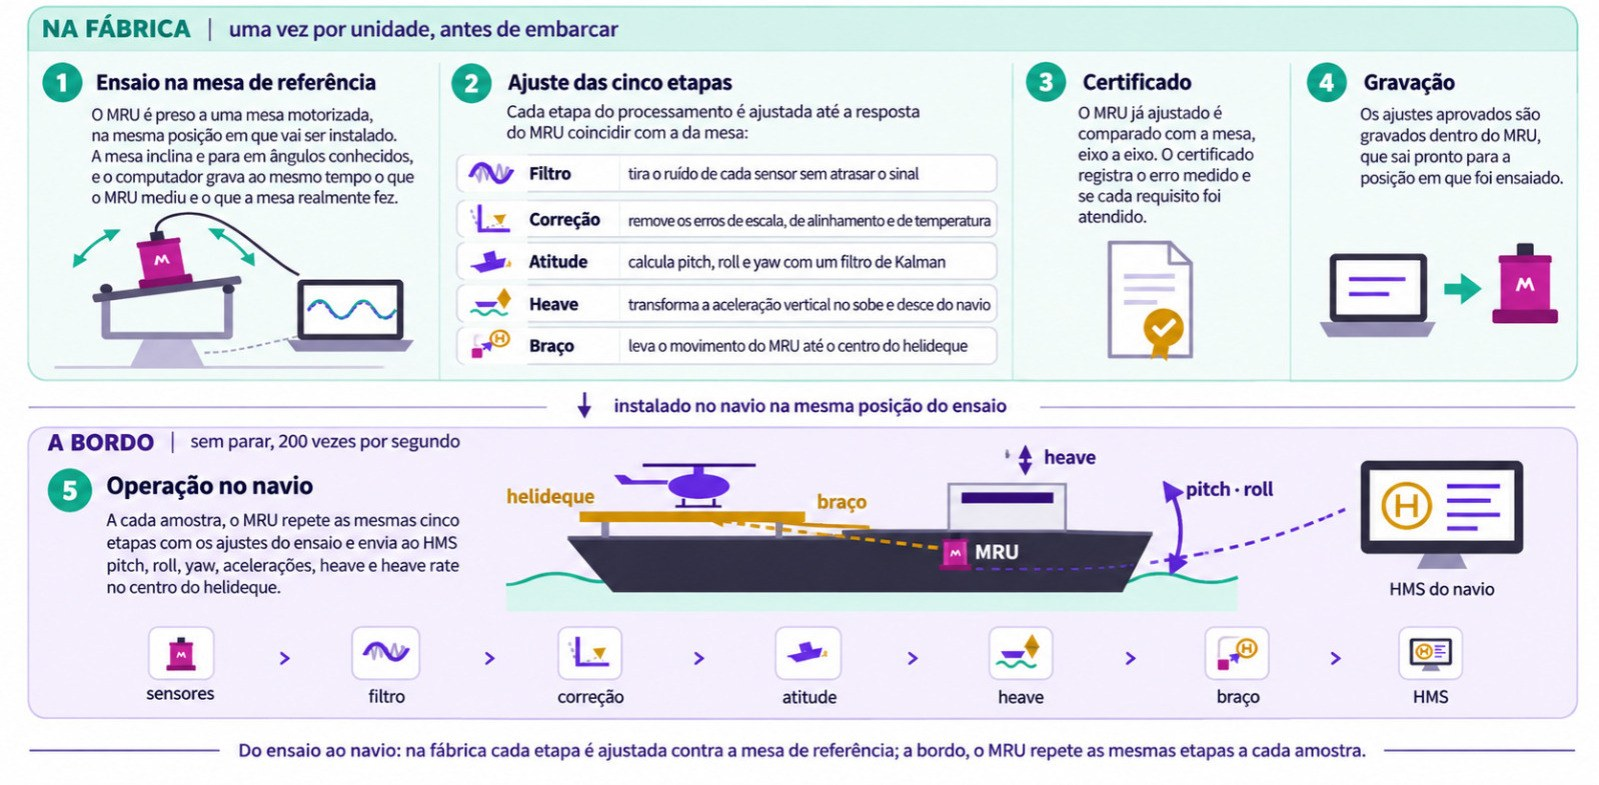
\includegraphics[width=\textwidth]{images/pipeline_esquematico.jpg}
    \fonte{Autoria Própria}
\end{figure}

No pré-processamento, os registros do MRU e da referência são reamostrados em uma grade de tempo comum, a defasagem entre os dois equipamentos é corrigida por correlação cruzada e os trechos em movimento e em repouso são separados. Em seguida, as cinco etapas do processamento (filtro, correção, atitude, \textit{heave} e braço, detalhadas na Seção~\ref{sec:pipeline}) são ajustadas até a resposta do MRU coincidir com a da mesa.

Os dados finais calibrados são comparados com a referência, eixo a eixo, e o certificado de calibração registra o erro medido e se cada requisito foi atendido. Os ajustes aprovados são gravados no próprio MRU, que, a bordo, repete as mesmas etapas a cada amostra e envia ao HMS \textit{pitch}, \textit{roll}, \textit{yaw}, acelerações, \textit{heave} e \textit{heave rate} no centro do helideque.

\newpage
\section{Entregas do Projeto}\label{sec:entregas}

Nesta seção, são detalhados os processos e resultados referentes ao escopo desta macroentrega, estruturados conforme os produtos e critérios de aceitação estabelecidos no Plano de Trabalho.

\subsection{Mapeamento de Lacunas (\textit{Gap Analysis})}

\subsubsection{Estado Atual}

O ciclo I resultou no Measure MRU apresentado na Figura~\ref{fig:fotosmru}. O equipamento reúne, em um invólucro cilíndrico de alumínio usinado e anodizado, duas placas de circuito impresso empilhadas, a de alimentação e a de sensores e comunicação, o processador ESP32-S3 e o sensor inercial KERNEL-120, com as interfaces RS-422 e RS-232 disponíveis em um conector circular de 8 vias. O \textit{firmware} embarcado executa a leitura do sensor, a filtragem e a fusão dos dados, e cada unidade é calibrada individualmente e acompanhada de certificado de calibração.

\begin{figure}[H]
    \centering
    \caption{Fotos do MRU Measure}
    \label{fig:fotosmru}
    \subfloat[]{
        \frame{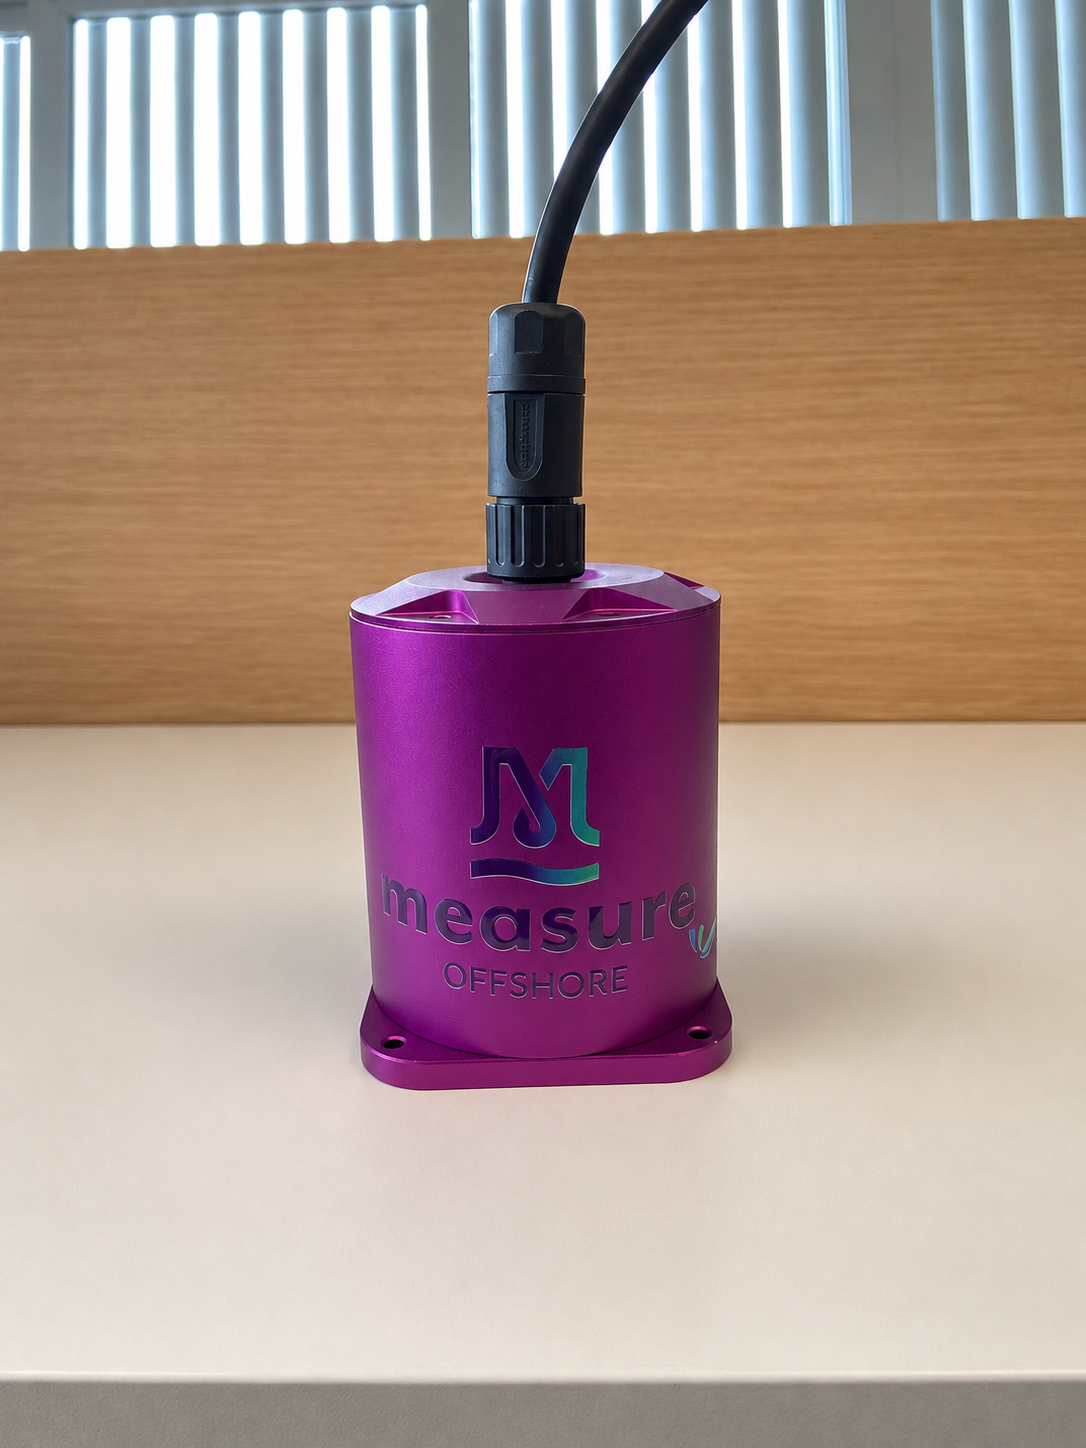
\includegraphics[height=7cm]{images/Purple MRU Device on Minimal Desk.png}}
    }\hfill\subfloat[]{
        \frame{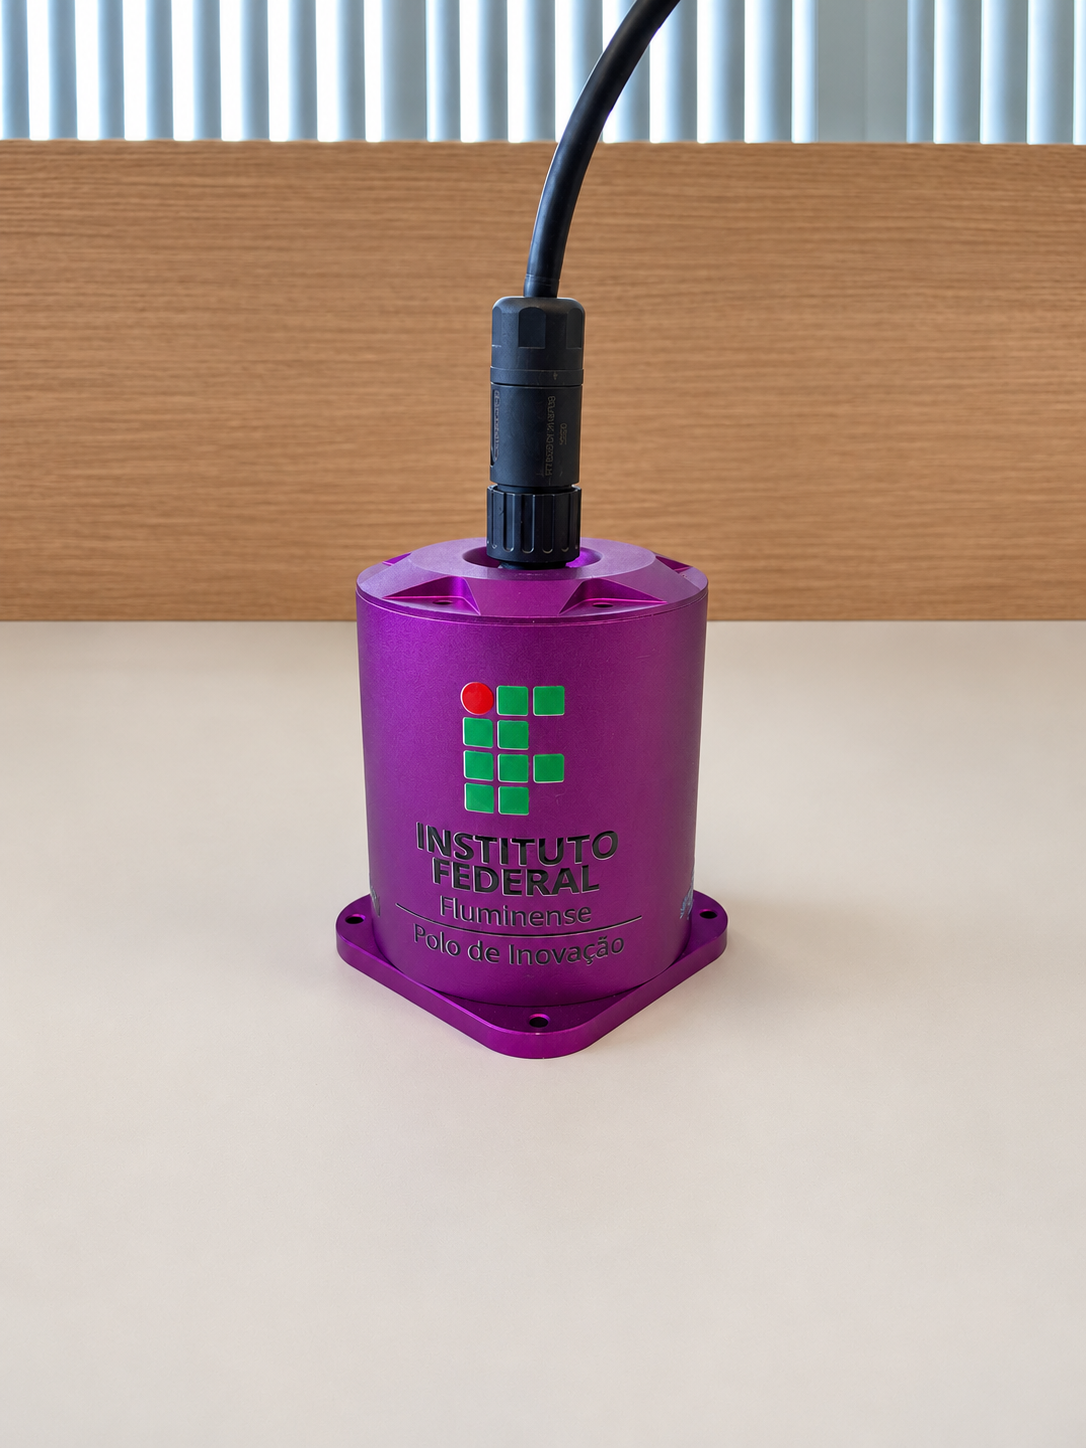
\includegraphics[height=7cm]{images/Purple MRU Device on Cream Tabletop.png}}
    }\hfill\subfloat[]{
        \frame{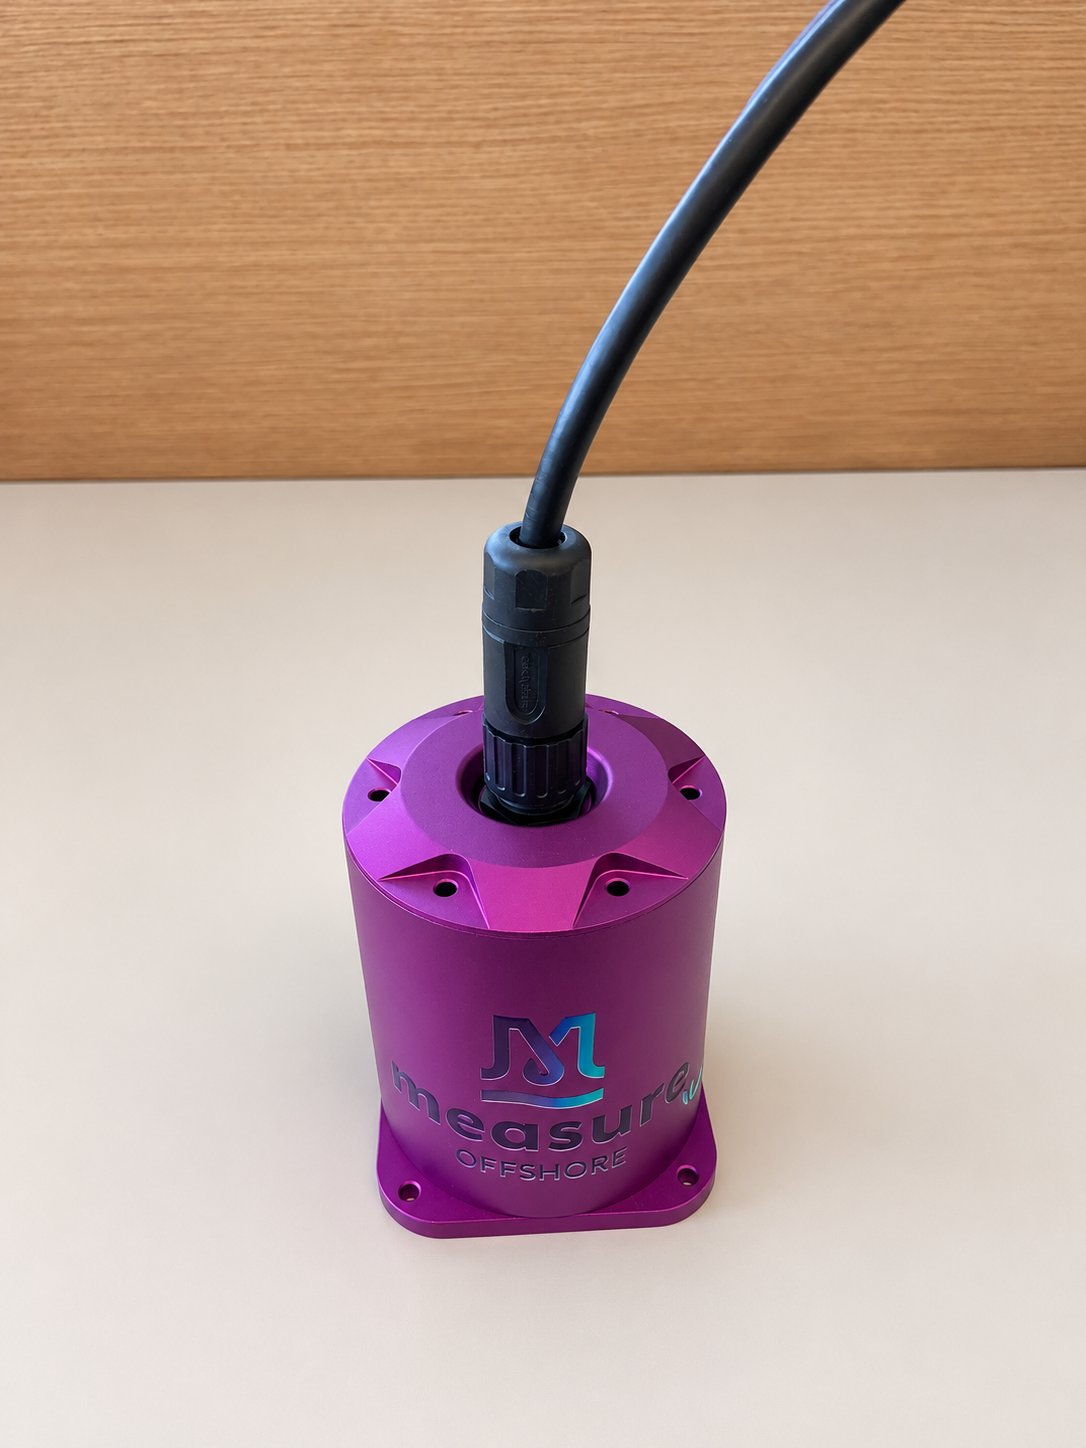
\includegraphics[height=7cm]{images/Purple Measure Offshore Device on Desk.png}}
    }
    \fonte{Autoria Própria}
\end{figure}

A extração dos dados é feita pelo conector circular de 8 vias, que reúne a alimentação em corrente contínua e as duas interfaces seriais: a RS-422, diferencial e \textit{full-duplex}, que é o canal de dados do HMS, e a RS-232, usada para configuração, diagnóstico e transmissão local; uma porta USB de serviço atende ao uso em bancada. O \textit{firmware} transmite as grandezas em JSON, em lista (LIST) ou na sentença NMEA 0183 \texttt{\$GPPASHR}, com taxa configurável até 100~Hz. No computador, o software de monitoramento (HMS) desenvolvido pela equipe recebe esse fluxo, exibe \textit{roll}, \textit{pitch} e \textit{yaw} em tempo real e permite exportar os dados em JSON ou CSV para análise, como na bancada da Figura~\ref{fig:plataforma}. O modo de aquisição é usado nos ensaios de calibração (Seção~\ref{sec:metodologia}).

\begin{figure}[H]
    \centering
    \caption{Fotos do MRU com plataforma de Monitoramento}
    \label{fig:plataforma}
    \frame{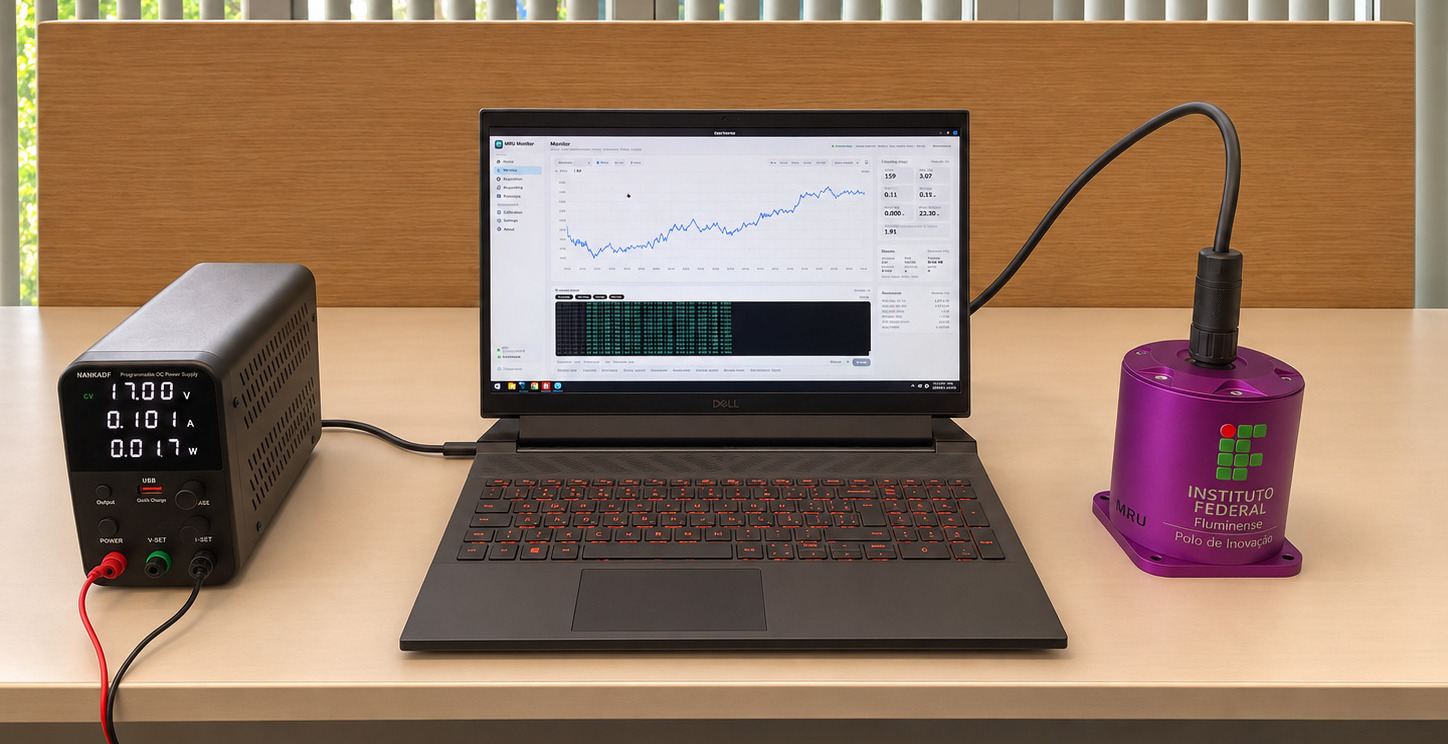
\includegraphics[width=0.8\linewidth]{images/WhatsApp Image 2026-11-05 at 14.39.34.jpeg}}
    \fonte{Autoria Própria}
\end{figure}

O invólucro desse equipamento foi projetado para estanqueidade, sem juntas à prova de chama, e o conector externo não tem certificação Ex. Essas características são consolidadas na linha de base apresentada a seguir.

\subsubsection{Linha de Base: Protótipo da Fase Anterior}

A Tabela~\ref{tab:linhabase} resume as características do protótipo consolidado na fase anterior, conforme registrado no manual técnico e de instalação do dispositivo \cite{manualdrmm} e na lista oficial de componentes (BOM v2).

\begin{table}[H]
    \centering
    \caption{Características do protótipo da fase anterior}
    \label{tab:linhabase}
    \renewcommand{\arraystretch}{1.3}
    \begin{tabularx}{\textwidth}{|>{\raggedright\arraybackslash}p{3.6cm}|>{\raggedright\arraybackslash}X|}
        \hline
        \centering\arraybackslash\textbf{Característica} & \centering\arraybackslash\textbf{Protótipo da fase anterior} \\ \hline
        Invólucro & Cilíndrico, com base de fixação quadrada, em alumínio anodizado com tratamento para resistência à corrosão \\ \hline
        Dimensões e massa & \O101,6~mm (diâmetro) $\times$ 126~mm (altura); base 101,6~mm $\times$ 101,6~mm; massa total 451,6~g \\ \hline
        Vedação & Grau de proteção IP66, utilizando gaxetas de silicone e prensa-cabos estanque \\ \hline
        Conector & Circular militar de 8 vias (série RTS6BS12N8P03), sem certificação Ex \\ \hline
        Fixação & 4 parafusos M5 na base \\ \hline
        Alimentação & 16~V a 29~V c.c. \\ \hline
        Consumo & Aproximadamente 3,6~W (18~V $\times$ 0,2~A) \\ \hline
        Comunicação & RS-422 e RS-232; protocolo NMEA 0183; frequência de saída configurável até 100~Hz \\ \hline
        Processamento & Unidade \textit{dual-core} de 32 bits (placa ESP32-S3-Zero) \\ \hline
        Sensoriamento & AHRS baseado em sensores MEMS de grau tático (Inertial Labs KERNEL-120) \\ \hline
        Placas eletrônicas & Placa de alimentação (\textit{Mainboard} v0.1, com conversor c.c.-c.c. TMR~6-2411) e placa de sensores e comunicação (\textit{Sensorboard} v0.2), interligadas por barras de pinos de 2,54~mm sem trava \\ \hline
        Proteção da entrada & MOSFET contra inversão de polaridade e varistor de 39~V; sem fusível \\ \hline
        Isolamento galvânico & Previsto no projeto para a RS-422 (fonte isolada MAX253 com transformador e isolador digital ADuM3301), mas fora da especificação, pois a fonte isolada, sem regulação, chegava a 6--10~V em circuitos integrados de 5,5~V, e não montado na BOM v2 \\ \hline
        Proteção Ex & Não possui: invólucro projetado para estanqueidade, sem juntas à prova de chama, e equipamento sem certificação \\ \hline
    \end{tabularx}
    \fonte{Autoria Própria}
\end{table}

A linha de base mostra que parte do protótipo pode ser aproveitada: o invólucro metálico já atende aos requisitos de proteção contra cargas eletrostáticas e de grau de proteção, e a potência dissipada, de cerca de 3,6~W, é compatível com a classe de temperatura T4. As lacunas concentram-se na proteção da entrada de alimentação, que não possui fusível, na retenção das conexões internas, no módulo processador com botões e porta USB, no conector externo sem certificação Ex e na ausência de terminal de aterramento e de marcação. Essas lacunas são detalhadas nas seções seguintes.

\subsubsection{Classificação-Alvo}\label{sec:classalvo}

A classificação-alvo reúne o tipo de proteção, o nível de proteção do equipamento (EPL), o grupo de gás e a classe de temperatura que o DRMM deve atender. Quem define a zona do local de instalação é a operadora, no desenho de classificação de áreas, e o equipamento é escolhido para a zona. A classificação de áreas segue a ABNT NBR IEC 60079-10-1: a Zona~1 exige EPL Gb, e a Zona~2 admite EPL Gc. O DRMM é instalado sob o centro do helideque, próximo ao abastecimento de aeronaves e a equipamentos de processo, e a zona desse local ainda não foi informada, razão pela qual a análise cobre as duas situações. Para o grupo de gás, adotou-se o IIC, escolha conservadora que abrange os grupos IIA e IIB; o IIA é o típico de plataformas de óleo e gás. Para a temperatura, adotou-se a classe T4 (135~°C), a mais comum em plataformas, que o equipamento, com consumo de cerca de 3,6~W, atende com folga.

A Tabela~\ref{tab:tiposprotecao} compara os tipos de proteção quanto ao que precisa mudar na eletrônica em cada um. O Ex d e o Ex ec foram avaliados item a item (Seção~\ref{sec:planilha}); os demais tipos não.

{\footnotesize
\renewcommand{\arraystretch}{1.25}
\begin{longtable}{|>{\raggedright\arraybackslash}p{2.0cm}|>{\raggedright\arraybackslash}p{1.6cm}|>{\raggedright\arraybackslash}p{1.4cm}|>{\raggedright\arraybackslash}p{3.5cm}|>{\raggedright\arraybackslash}p{3.3cm}|>{\raggedright\arraybackslash}p{1.85cm}|}
    \caption{Comparativo dos tipos de proteção: impacto na eletrônica}\label{tab:tiposprotecao}\\
    \hline
    \centering\arraybackslash\textbf{Tipo de proteção} & \centering\arraybackslash\textbf{Norma} & \centering\arraybackslash\textbf{Zona / EPL} & \centering\arraybackslash\textbf{Mudanças necessárias na eletrônica} & \centering\arraybackslash\textbf{Principal impedimento / observações} & \centering\arraybackslash\textbf{Decisão} \\ \hline
    \endfirsthead
    \hline
    \centering\arraybackslash\textbf{Tipo de proteção} & \centering\arraybackslash\textbf{Norma} & \centering\arraybackslash\textbf{Zona / EPL} & \centering\arraybackslash\textbf{Mudanças necessárias na eletrônica} & \centering\arraybackslash\textbf{Principal impedimento / observações} & \centering\arraybackslash\textbf{Decisão} \\ \hline
    \endhead
    \multicolumn{6}{r}{\textit{continua na próxima página}} \\
    \endfoot
    \endlastfoot
    Ex d / Ex db (invólucro à prova de explosão) & ABNT NBR IEC 60079-1 & Zona 1 e 2 / Gb & Nenhuma mudança obrigatória por ignição (a explosão interna é contida). Mudanças adotadas por confiabilidade: fusível, varistor 07D470K, zener no Q1, fonte de 12~V para o KERNEL, conectores com trava & Os 2 itens que não atendem: proteção da entrada (resolvida pelas mudanças adotadas) e entrada de cabos (prensa-cabo Ex d, fora da eletrônica). Variante Ex db eb: compartimento de terminais em segurança aumentada, sem impacto na eletrônica & Alvo (Zona~1) \\ \hline
    Ex ec (segurança aumentada) & ABNT NBR IEC 60079-7 & Zona 2 / Gc & Trocar ESP32-S3-Zero por módulo soldado (ESP32-S3-WROOM-1); fusível; varistor 07D470K; zener no Q1; fonte de 12~V para o KERNEL; ADM2587E no lugar da fonte isolada MAX253; conectores Molex com trava; revisão de distâncias de isolação e verniz & Hoje a placa tem partes que podem faiscar (botões e USB do ESP, \textit{jumpers}) e componentes fora dos valores nominais (Q1, varistor, KERNEL, fonte isolada). Todos os itens têm solução definida (Tabela~\ref{tab:alteracoes}) & Alvo (Zona~2) \\ \hline
    Ex nR (respiração restrita) & ABNT NBR IEC 60079-15 & Zona 2 / Gc & Proteção da entrada (fusível, varistor, zener no Q1) e fonte de 12~V para o KERNEL. O ESP e os conectores podem ficar, pois a proteção é feita pela vedação do invólucro & A proteção depende de o invólucro manter a vedação ao longo da vida útil (ensaio de respiração restrita e porta de teste). Exige controle de vedação em manutenção \textit{offshore} & Reserva (Zona~2) \\ \hline
    Ex ia / Ex ib (segurança intrínseca) & ABNT NBR IEC 60079-11 & Zona 0, 1 e 2 / Ga, Gb & Redesenho completo: limitar tensão, corrente e potência em todas as entradas (barreiras ou limitadores), limitar capacitâncias e indutâncias, isolação obrigatória entre circuitos, distâncias da 60079-11 e trocar o c.c.-c.c. & Consumo de $\sim$3,6~W, muito acima da potência disponível num circuito Ex i do grupo IIC (da ordem de 1~W ou menos). Só o KERNEL já consome $\sim$0,5~W & Descartado \\ \hline
    Ex ma / Ex mb (encapsulamento) & ABNT NBR IEC 60079-18 & Zona 0, 1 e 2 / Ga, Gb & Encapsular as placas (ou as partes que faíscam) em resina; usar componentes compatíveis com encapsulamento (sem cavidades, com limites para eletrolíticos); fusível de proteção obrigatório; controlar a temperatura dentro da resina & Sem acesso para manutenção e atualização de \textit{firmware}; o KERNEL e os conectores não podem ser encapsulados; o calor do c.c.-c.c. e do ADM2587E fica preso na resina & Descartado \\ \hline
    Ex px / Ex py / Ex pz (pressurização) & ABNT NBR IEC 60079-2 & Zona 1 e 2 / Gb, Gc & Adicionar o sistema de controle da pressurização: sensor de pressão ou fluxo, temporizador de purga e desligamento automático da alimentação & Exige suprimento contínuo de ar limpo ou gás inerte e monitoramento na plataforma, desproporcional para um sensor de $\sim$3,6~W & Descartado \\ \hline
\end{longtable}
}
{\vspace{-0.5\baselineskip}\fonte{Autoria Própria}\par}

Os tipos-alvo do DRMM são, portanto, o Ex ec, para Zona~2, e o Ex d (Ex db), para Zona~1, com o Ex nR como reserva para Zona~2. A Tabela~\ref{tab:alvo} apresenta a classificação-alvo correspondente a cada caso.

\begin{table}[H]
    \centering
    \caption{Classificação-alvo do DRMM para atmosferas explosivas}
    \label{tab:alvo}
    \renewcommand{\arraystretch}{1.3}
    \begin{tabularx}{\textwidth}{|>{\raggedright\arraybackslash}p{3.4cm}|>{\raggedright\arraybackslash}X|>{\raggedright\arraybackslash}X|}
        \hline
        \centering\arraybackslash\textbf{Parâmetro} & \centering\arraybackslash\textbf{Zona 1} & \centering\arraybackslash\textbf{Zona 2} \\ \hline
        Tipo de proteção & Invólucro à prova de explosão ``d'' (Ex db; variante Ex db eb, com compartimento de terminais em segurança aumentada) & Segurança aumentada ``e'' (Ex ec) \\ \hline
        Norma específica & ABNT NBR IEC 60079-1:2016 & ABNT NBR IEC 60079-7:2018 \\ \hline
        Nível de proteção (EPL) & Gb & Gc \\ \hline
        Grupo de gás & IIC & IIC \\ \hline
        Classe de temperatura & T4 (135~°C) & T4 (135~°C) \\ \hline
        Temperatura ambiente & $-20$~°C a $+60$~°C (proposta) & $-20$~°C a $+60$~°C (proposta) \\ \hline
        Marcação & Ex db IIC T4 Gb & Ex ec IIC T4 Gc \\ \hline
        Grau de proteção & -- & Mínimo IP54 \\ \hline
        Entrada de cabos e conector externo & Prensa-cabo Ex d certificado com cabo fixo (ou conector com certificação Ex d) & Conector aceito com trava, grau IP e etiqueta ``Não desconectar energizado'' \\ \hline
    \end{tabularx}
    \fonte{Autoria Própria}
\end{table}

Durante o estudo, verificou-se que os MRUs comerciais de referência, como o MRU 5 da Kongsberg e os sensores da Inertial Labs e da Xsens, não possuem certificação Ex. O manual de instalação do HMS 300 da Kongsberg orienta que, em helideque localizado em zona Ex, a unidade inercial seja montada em uma caixa Ex, e a única solução de MRU completo com certificação encontrada no mercado é a de uma unidade comum instalada em caixa de alumínio Ex d certificada, da SMC, com cerca de 43~kg e marcação Ex d IIB T6 Gb. Com isso, abriu-se a discussão entre incorporar a proteção Ex ao próprio DRMM, o que constituiria um diferencial frente aos concorrentes, ou indicar um invólucro Ex à parte, como fazem os demais fabricantes. O estudo de certificação recomenda, em qualquer caso, projetar a placa já pensando no Ex ec, pois ela continua servindo dentro de um invólucro Ex d. Para a Zona~2, a Portaria Inmetro nº 115/2022 admite ainda a instalação sem certificação de equipamento que não produza faíscas nem superfícies quentes e esteja em invólucro adequado (Art.~3º, §~2º, III), decisão que cabe ao responsável pela instalação e que as operadoras costumam condicionar ao certificado.

\subsubsection{Planilha de Mapeamento de Requisitos Normativos}\label{sec:planilha}

A Tabela~\ref{tab:gap} apresenta a avaliação da eletrônica frente aos dois tipos de proteção, com a classificação-alvo Ex db IIC T4 Gb (Zona~1) e Ex ec IIC T4 Gc (Zona~2). Para cada requisito, a planilha registra a situação atual da eletrônica, a avaliação e a ação ou decisão tomada. Os itens gerais (ABNT NBR IEC 60079-0) valem para os dois tipos de proteção, e os itens específicos valem só para o Ex d (ABNT NBR IEC 60079-1) ou só para o Ex ec (ABNT NBR IEC 60079-7).

{\footnotesize
\renewcommand{\arraystretch}{1.25}
\begin{longtable}{|>{\centering\arraybackslash}p{0.6cm}|>{\raggedright\arraybackslash}p{2.8cm}|>{\raggedright\arraybackslash}p{4.0cm}|>{\raggedright\arraybackslash}p{1.7cm}|>{\raggedright\arraybackslash}p{4.2cm}|}
    \caption{Mapeamento de requisitos normativos: avaliação da eletrônica para Ex d e Ex ec}\label{tab:gap}\\
    \hline
    \textbf{\#} & \centering\arraybackslash\textbf{Requisito} & \centering\arraybackslash\textbf{Situação atual da eletrônica} & \centering\arraybackslash\textbf{Avaliação} & \centering\arraybackslash\textbf{Ação / decisão tomada} \\ \hline
    \endfirsthead
    \hline
    \textbf{\#} & \centering\arraybackslash\textbf{Requisito} & \centering\arraybackslash\textbf{Situação atual da eletrônica} & \centering\arraybackslash\textbf{Avaliação} & \centering\arraybackslash\textbf{Ação / decisão tomada} \\ \hline
    \endhead
    \multicolumn{5}{r}{\textit{continua na próxima página}} \\
    \endfoot
    \endlastfoot
    \multicolumn{5}{|l|}{\textbf{Requisitos gerais (valem para Ex d e Ex ec) --- ABNT NBR IEC 60079-0}} \\ \hline
    G1 & Classe de temperatura T4: nenhuma superfície acima de 135~°C & Potência total $\approx$~3,6~W (18~V $\times$ 0,2~A). Pontos mais quentes: KERNEL-120 ($\approx$~80~°C estimado), conversor TMR~6-2411 e, após a troca, ADM2587E (até 0,65~W). Bem abaixo de 135~°C & \avA & Confirmar por medição com a caixa fechada na temperatura ambiente máxima declarada \\ \hline
    G2 & Faixa de temperatura ambiente declarada & KERNEL-120 opera de $-40$~°C a $+85$~°C; demais componentes industriais. Faixa do equipamento ainda não declarada & \avJ & Declarar a faixa na marcação (proposta: $-20$~°C a $+60$~°C, por estar sob o helideque ao sol) \\ \hline
    G3 & Fontes de radiofrequência abaixo da potência-limite do grupo de gás & Rádio Wi-Fi/BLE do ESP32-S3 com $\sim$0,1~W (20~dBm), muito abaixo do limite para o grupo IIC & \avA & Desligar o rádio no \textit{firmware} se não for usado \\ \hline
    G4 & Células e baterias & O MRU não possui baterias & \avNA & -- \\ \hline
    G5 & Proteção da alimentação de entrada contra sobrecorrente e sobretensão (ABNT NBR IEC 60079-0 e 60079-14) & Sem fusível. Em uma falha da fonte ($\approx$~50~V), o Q1 e o KERNEL queimaram; o KERNEL recebe a entrada sem regulação & \avN & Fusível T500~mA com porta-fusível com tampa; varistor 07D470K; zener no \textit{gate} do Q1; fonte RECOM de 12~V para o KERNEL (Tabela~\ref{tab:alteracoes}) \\ \hline
    G6 & Documentação técnica: desenhos e lista de componentes controlados (ABNT NBR IEC 60079-0 e Portaria Inmetro nº 115/2022) & Esquemáticos Altium e BOM v2 existem, ainda sem controle de revisão para Ex & \avJ & Criar série de desenhos Ex e lista de componentes críticos com controle de mudanças \\ \hline
    \multicolumn{5}{|l|}{\textbf{Requisitos específicos do Ex d --- ABNT NBR IEC 60079-1}} \\ \hline
    D1 & Componentes eletrônicos dentro do invólucro à prova de explosão & No Ex d, a ignição interna é contida pelo invólucro: botões, conectores e o ESP32-S3-Zero não precisam ser trocados por motivo de ignição & \avA & -- \\ \hline
    D2 & Temperatura da superfície externa do invólucro & Caixa de alumínio usinado conduz bem o calor dos $\sim$3,6~W internos & \avA & Medir no ensaio de tipo (item G1) \\ \hline
    D3 & Arranjo interno: não subdividir o volume (evitar pressão em cascata) & Duas placas empilhadas com espaçadores, sem divisórias fechadas & \avV & Manter as placas abertas (sem compartimentos); o OCP avalia no ensaio de sobrepressão \\ \hline
    D4 & Entrada de cabos e conector externo (ABNT NBR IEC 60079-1 e 60079-14) & Conector circular RTS712ND8S03 sem certificação Ex d & \avN & Prensa-cabo Ex d certificado com cabo fixo (ou conector com certificação Ex d) \\ \hline
    D5 & Conectores internos entre placas (boa prática, vibração) & Barras de pinos Samtec de 2,54~mm sem trava. Não é exigido no Ex d & \avJ & Trocar por Molex Micro-Fit com trava e cabo pronto (a mesma placa serve para Ex d e Ex ec) \\ \hline
    D6 & Isolamento galvânico da serial RS-422 (não exigido pela ABNT NBR IEC 60079-1) & Fonte isolada atual (MAX253) fora da especificação: até 10~V em CIs de 5,5~V & \avNA & Melhoria funcional: troca pelo ADM2587E (Tabela~\ref{tab:alteracoes}) \\ \hline
    \multicolumn{5}{|l|}{\textbf{Requisitos específicos do Ex ec --- ABNT NBR IEC 60079-7}} \\ \hline
    E1 & Nenhuma faísca ou arco em operação normal & ESP32-S3-Zero é placa de desenvolvimento com botões BOOT/RESET e USB-C; J1 da \textit{Sensorboard} usa \textit{jumpers} removíveis & \avN & Trocar por módulo ESP32-S3 soldado e blindado (ESP32-S3-WROOM-1); J1 eliminado com o ADM2587E \\ \hline
    E2 & Componentes usados dentro dos seus valores nominais & Q1: \textit{gate} de $\pm$20~V recebendo 24--36~V. Varistor 07D390K: 31~V c.c. para entrada de até 36~V. KERNEL: máximo de 30~V recebendo até 36~V. Fonte isolada MAX253: até 10~V em CIs de 5,5~V. RX da RS-422 em 5~V no ESP32 (3,3~V) & \avN & Zener de 15~V e R1 de 47~k$\Omega$ no Q1; varistor 07D470K; RECOM de 12~V no KERNEL; ADM2587E em 3,3~V; C13 de 63~V \\ \hline
    E3 & Proteção contra sobrecorrente (aquecimento em falha) & Não há fusível na entrada & \avN & Fusível de vidro 5$\times$20~mm T500~mA 250~V em porta-fusível de placa com tampa, antes do varistor \\ \hline
    E4 & Fusível adequado ao Ex ec (encapsulado, não religável) & Fusível de vidro em porta-fusível com tampa (decisão nova) & \avV & Confirmar com o OCP na pré-avaliação; alternativa: fusível cerâmico ou PTC \\ \hline
    E5 & Ligações internas que não se soltam (conectores com retenção) & Barras de pinos e soquetes Samtec de 2,54~mm sem trava; placas fixadas por espaçadores & \avN & Molex Micro-Fit 3.0 com trava (43045-1012) e cabo pronto de fábrica; espaçadores M3 de 25~mm \\ \hline
    E6 & Distâncias de isolação na placa (escoamento e separação) & \textit{Layout} não revisado para Ex; tensão máxima de 36~V & \avV & Revisar as distâncias na próxima revisão do \textit{layout} e aplicar verniz conformal \\ \hline
    E7 & Grau de proteção do invólucro (mínimo IP54) & Caixa de alumínio projetada para IP68 & \avA & Confirmar no ensaio de tipo \\ \hline
    E8 & Conector externo (ABNT NBR IEC 60079-7 e 60079-14) & Conector circular RTS712ND8S03 sem certificação Ex, com vedação & \avJ & Aceito com trava, grau IP e etiqueta ``Não desconectar energizado'' \\ \hline
    E9 & Temperatura dos componentes internos (o gás entra no invólucro) & Componentes mais quentes estimados bem abaixo de 135~°C (item G1) & \avV & Medir o ponto mais quente dentro da caixa fechada (KERNEL, TMR, ADM2587E, RECOM) \\ \hline
\end{longtable}
}
{\vspace{-0.5\baselineskip}\fonte{Autoria Própria}\par}

No Ex d, dos 12 itens, 4 atendem, 3 atendem com ajuste, 2 não atendem, 1 está a verificar e 2 não se aplicam. No Ex ec, dos 15 itens, 3 atendem, 3 atendem com ajuste, 5 não atendem, 3 estão a verificar e 1 não se aplica. É uma contagem: os itens têm pesos diferentes e não devem ser lidos como porcentagem de conformidade.

\subsection{Modelagem em CAD 3D do Novo Invólucro à Prova de Explosão Tipo ``d''}\label{sec:cad}

O novo invólucro foi desenvolvido em três protótipos digitais, modelados em CAD 3D, que diferem na forma de fechamento: o primeiro tem parafusos verticais na tampa e na base, o segundo tem parafusos horizontais na lateral e o terceiro tem fechamento rosqueado. Os três foram projetados considerando os requisitos de proteção contra explosão Ex d e o grau de proteção IP66 e possuem encaixes antierro. A Figura~\ref{fig:cad} apresenta os modelos.

\begin{figure}[H]
    \centering
    \caption{Protótipos CAD 3D do invólucro à prova de explosão do DRMM}
    \label{fig:cad}
    % PENDENTE: imagens dos três protótipos (cobrar Yuri)
    \reservado{5cm}{(inserir imagens dos três protótipos CAD: parafusos verticais, parafusos horizontais e fechamento rosqueado)}
    \fonte{Autoria Própria}
\end{figure}

Em reunião com a empresa responsável pela usinagem, o modelo com parafusos verticais recebeu a melhor avaliação, embora alguns pontos ainda precisem ser ajustados. Para o material, foi considerado o alumínio 6061-T5, com parede do cilindro de 8~mm. A Tabela~\ref{tab:dimensoes} resume os principais parâmetros dimensionais e a fixação de cada alternativa.

\begin{table}[H]
    \centering
    \caption{Principais parâmetros dimensionais do invólucro}
    \label{tab:dimensoes}
    \renewcommand{\arraystretch}{1.3}
    \begin{tabularx}{\textwidth}{|>{\raggedright\arraybackslash}p{5.2cm}|>{\raggedright\arraybackslash}X|}
        \hline
        \centering\arraybackslash\textbf{Parâmetro} & \centering\arraybackslash\textbf{Valor} \\ \hline
        Altura total (da tampa à base) & 120,3~mm \\ \hline
        Altura do cilindro & 108~mm \\ \hline
        Diâmetro externo do cilindro & 101,6~mm \\ \hline
        Diâmetro interno do cilindro & 85,45~mm \\ \hline
        Espessura da parede do cilindro & 8~mm \\ \hline
        Altura da base e da sua borda & 18~mm e 6~mm \\ \hline
        Altura da tampa e da sua borda & 12,5~mm e 6~mm \\ \hline
        Material & Alumínio 6061-T5 (considerado) \\ \hline
        Fixação: parafusos verticais & Tampa: 6 $\times$ M4$\times$0,7, L = 12~mm; base: 6 $\times$ M4$\times$0,7, L = 12~mm; suporte: 8 $\times$ M6$\times$1, L = 12~mm \\ \hline
        Fixação: parafusos horizontais & Lateral: 8 $\times$ M4$\times$0,7, L = 12~mm; suporte: 8 $\times$ M6$\times$1, L = 12~mm \\ \hline
        Fixação: fechamento rosqueado \pendente{(confirmar com a mecânica)} & Tampa: 1 $\times$ M3$\times$0,5, L = 10~mm; base: 1 $\times$ M3$\times$0,5, L = 10~mm; suporte: 8 $\times$ M6$\times$1, L = 12~mm \\ \hline
    \end{tabularx}
    \fonte{Autoria Própria}
\end{table}

A Tabela~\ref{tab:arquivos} relaciona os arquivos de modelagem digital e os desenhos técnicos em PDF extraídos diretamente do software.

\begin{table}[H]
    \centering
    \caption{Arquivos de modelagem entregues}
    \label{tab:arquivos}
    \renewcommand{\arraystretch}{1.3}
    \begin{tabularx}{\textwidth}{|>{\raggedright\arraybackslash}p{5.2cm}|>{\centering\arraybackslash}p{2.2cm}|>{\raggedright\arraybackslash}X|}
        \hline
        \centering\arraybackslash\textbf{Arquivo} & \textbf{Formato} & \centering\arraybackslash\textbf{Conteúdo} \\ \hline
        % PENDENTE: nomes, formatos e conteúdo dos arquivos (Yuri)
        \pendente{[nome do arquivo]} & \pendente{[formato]} & \pendente{[conteúdo]} \\ \hline
        \pendente{[nome do arquivo]} & \pendente{[formato]} & \pendente{[conteúdo]} \\ \hline
        \pendente{[nome do arquivo]} & \pendente{[formato]} & \pendente{[conteúdo]} \\ \hline
        \pendente{[nome do arquivo]} & \pendente{[formato]} & \pendente{[conteúdo]} \\ \hline
    \end{tabularx}
    \fonte{Autoria Própria}
\end{table}

A definição do invólucro ainda não está firmada. Como os concorrentes não têm o invólucro Ex embutido e normalmente utilizam uma caixa à parte com proteção Ex, está em discussão se o DRMM deve ter um invólucro Ex por padrão e, nesse caso, qual tipo de proteção seria compatível com o projeto, ou se deve ser indicado um invólucro Ex à parte, como fazem os concorrentes.

\subsection{Simulação de Estresse Mecânico e Térmico via Software -- Métodos Clássicos}\label{sec:simulacao}

O comportamento térmico do DRMM foi avaliado pelo registro contínuo, por cerca de 12 horas, da temperatura interna do sensor KERNEL, medida pelo sensor de temperatura embutido no próprio componente, com o equipamento energizado dentro do invólucro. A Figura~\ref{fig:temperatura} apresenta a resposta obtida.

\begin{figure}[H]
    \centering
    \caption{Resposta térmica do sensor KERNEL com o equipamento energizado}
    \label{fig:temperatura}
    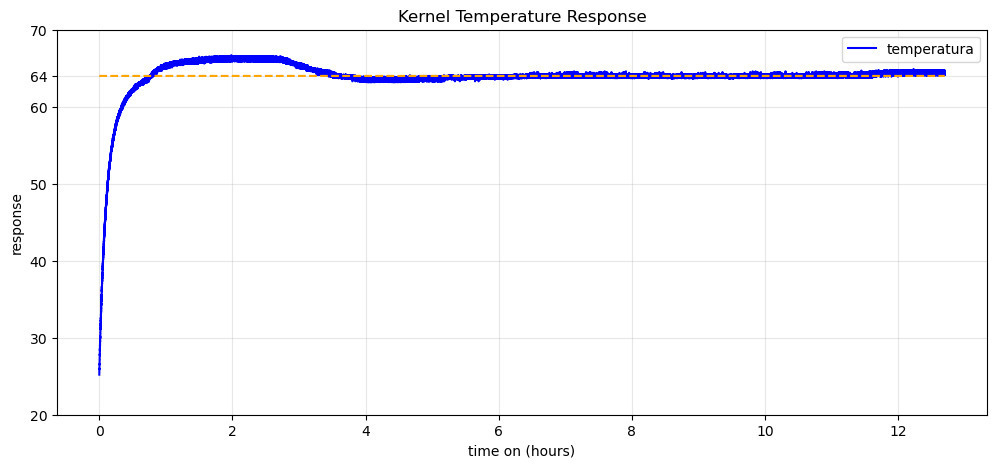
\includegraphics[width=0.95\textwidth]{images/temperatura_kernel.jpg}
    \fonte{Autoria Própria}
\end{figure}

Ao energizar o equipamento, a temperatura parte do valor ambiente, de cerca de 25~°C, e sobe rapidamente, ultrapassando 60~°C em menos de meia hora. Entre 1~h e 3~h, a curva apresenta um patamar pouco acima de 65~°C e, a partir de cerca de 4~h, estabiliza em torno de 64~°C, valor mantido até o fim do registro. A temperatura estabilizada está dentro da faixa de atuação do KERNEL, o que torna o resultado promissor, embora a dissipação de temperatura ainda vá ser melhorada.

% PENDENTE: curva térmica atualizada (Klauss) e premissas de cálculo da simulação mecânica e térmica (critério de aceitação da meta 2.3), a definir pela equipe.

\subsection{Adaptação dos Diagramas Esquemáticos e do Layout das PCBs com Isolamento Galvânico}\label{sec:pcb}

A adaptação da eletrônica partiu da avaliação da eletrônica frente aos tipos de proteção Ex d e Ex ec (Seção~\ref{sec:planilha}). Em uma falha da fonte de alimentação, de cerca de 50~V, o MOSFET de proteção Q1 e o KERNEL queimaram. As decisões da revisão de novembro de 2026 estão consolidadas na Tabela~\ref{tab:alteracoes}, que indica, para cada bloco do circuito, o componente atual, o componente adotado, o tipo de proteção que exige a troca e o motivo.

{\footnotesize
\renewcommand{\arraystretch}{1.25}
\begin{longtable}{|>{\raggedright\arraybackslash}p{2.0cm}|>{\raggedright\arraybackslash}p{3.0cm}|>{\raggedright\arraybackslash}p{3.4cm}|>{\raggedright\arraybackslash}p{1.7cm}|>{\raggedright\arraybackslash}p{3.2cm}|}
    \caption{Alterações de componentes das placas em relação à fase anterior}\label{tab:alteracoes}\\
    \hline
    \centering\arraybackslash\textbf{Bloco} & \centering\arraybackslash\textbf{Antes} & \centering\arraybackslash\textbf{Depois} & \centering\arraybackslash\textbf{Exigido para} & \centering\arraybackslash\textbf{Motivo} \\ \hline
    \endfirsthead
    \hline
    \centering\arraybackslash\textbf{Bloco} & \centering\arraybackslash\textbf{Antes} & \centering\arraybackslash\textbf{Depois} & \centering\arraybackslash\textbf{Exigido para} & \centering\arraybackslash\textbf{Motivo} \\ \hline
    \endhead
    \multicolumn{5}{r}{\textit{continua na próxima página}} \\
    \endfoot
    \endlastfoot
    Fusível de entrada & Nenhum & Fusível de vidro 5$\times$20~mm, T500~mA (retardado), 250~V, em porta-fusível de placa com tampa & Ex d e Ex ec & Proteção contra sobrecorrente; com o varistor, abre o circuito em sobretensão contínua \\ \hline
    Varistor de entrada & RV1 07D390K (39~V; cerca de 31~V c.c. contínuos) & 07D470K (47~V; cerca de 38~V c.c. contínuos) & Ex ec (recomendado no Ex d) & O 07D390K fica abaixo da tensão máxima de entrada (36~V) \\ \hline
    Proteção contra inversão & Q1 RQ5L015SP e R1 de 100~$\Omega$, com o \textit{gate} ligado ao GND & Q1 RQ5L015SP, zener de 15~V entre \textit{gate} e \textit{source} e R1 de 47~k$\Omega$ & Ex d e Ex ec & O \textit{gate} suporta $\pm$20~V e recebia toda a tensão de entrada (24--36~V), causa da queima do Q1 \\ \hline
    Capacitor de entrada & C13 de 220~\textmu F, 50~V & 220~\textmu F, 63~V & Ex ec (recomendado no Ex d) & Margem de tensão: ficou no limite \\ \hline
    Alimentação do KERNEL-120 & Ligação direta à entrada (18--36~V, sem regulação) & RECOM R-78HB12-0.5 (entrada de 17~V a 72~V, saída de 12~V fixos, 0,5~A) & Ex d e Ex ec & O KERNEL-120 aceita no máximo 30~V e queimou com a falha \\ \hline
    Isolamento da RS-422 & Fonte isolada MAX253 com transformador 78253/55MC e isolador ADuM3301, transceptor ADM489 e \textit{jumpers} em J1 & ADM2587E (RS-422/RS-485 isolado com fonte \textit{isoPower} integrada, 2,5~kV) & Ex ec (melhoria no Ex d) & A fonte isolada, sem regulação, chegava a 6--10~V em CIs de 5,5~V \\ \hline
    Processador & ESP32-S3-Zero (placa de desenvolvimento com botões e USB-C) & Módulo ESP32-S3-WROOM-1 soldado e blindado & Ex ec & Botões e conector USB podem gerar faísca em operação normal \\ \hline
    Conectores entre placas & Samtec TSW-104 e SSW-104, passo de 2,54~mm, sem trava & Molex Micro-Fit 3.0 (43045-1012) com cabo de fábrica (214755-1101) & Ex ec (recomendado no Ex d) & As ligações internas precisam de retenção contra vibração \\ \hline
    Conector externo & RTS712ND8S03 (circular, sem certificação Ex) & Ex d: prensa-cabo Ex d; Ex ec: Souriau 851-07A16-26P5016, com etiqueta ``Não desconectar energizado'' & Ex d & No Ex d, a entrada de cabos faz parte do invólucro à prova de explosão \\ \hline
    \textit{Layout} & Sem revisão para Ex & Revisão das distâncias de isolação e verniz conformal & Ex ec & Distâncias de escoamento e de isolação; proteção contra a maresia \\ \hline
\end{longtable}
}
{\vspace{-0.5\baselineskip}\fonte{Autoria Própria}\par}

A coluna ``Exigido para'' indica se a troca é exigida para o Ex d, para o Ex ec ou para ambos. O isolamento galvânico não é exigido pela norma.

\subsubsection{Antes: Placas da Fase Anterior}

Na fase anterior, a eletrônica do DRMM foi organizada em duas placas modulares, desenvolvidas no software Altium e fabricadas pela empresa Wego Sistemas: a placa de alimentação (\textit{Mainboard} v0.1) e a placa de sensores e comunicação (\textit{Sensorboard} v0.2), empilhadas com espaçadores e interligadas por barras de pinos. A Figura~\ref{fig:esq_ciclo1} apresenta o esquemático da placa de alimentação, que reúne a proteção contra inversão de polaridade (Q1), o varistor de entrada, o filtro de EMI, o conversor c.c.-c.c. isolado TMR~6-2411, de 18--36~V para 5~V, o supervisor de tensão e o estágio de fonte isolada para a RS-422, formado pelo \textit{driver} de transformador MAX253, pelo transformador 78253/55MC e pelos diodos SS14.

\begin{figure}[H]
    \centering
    \caption{Esquemático da placa de alimentação da fase anterior}
    \label{fig:esq_ciclo1}
    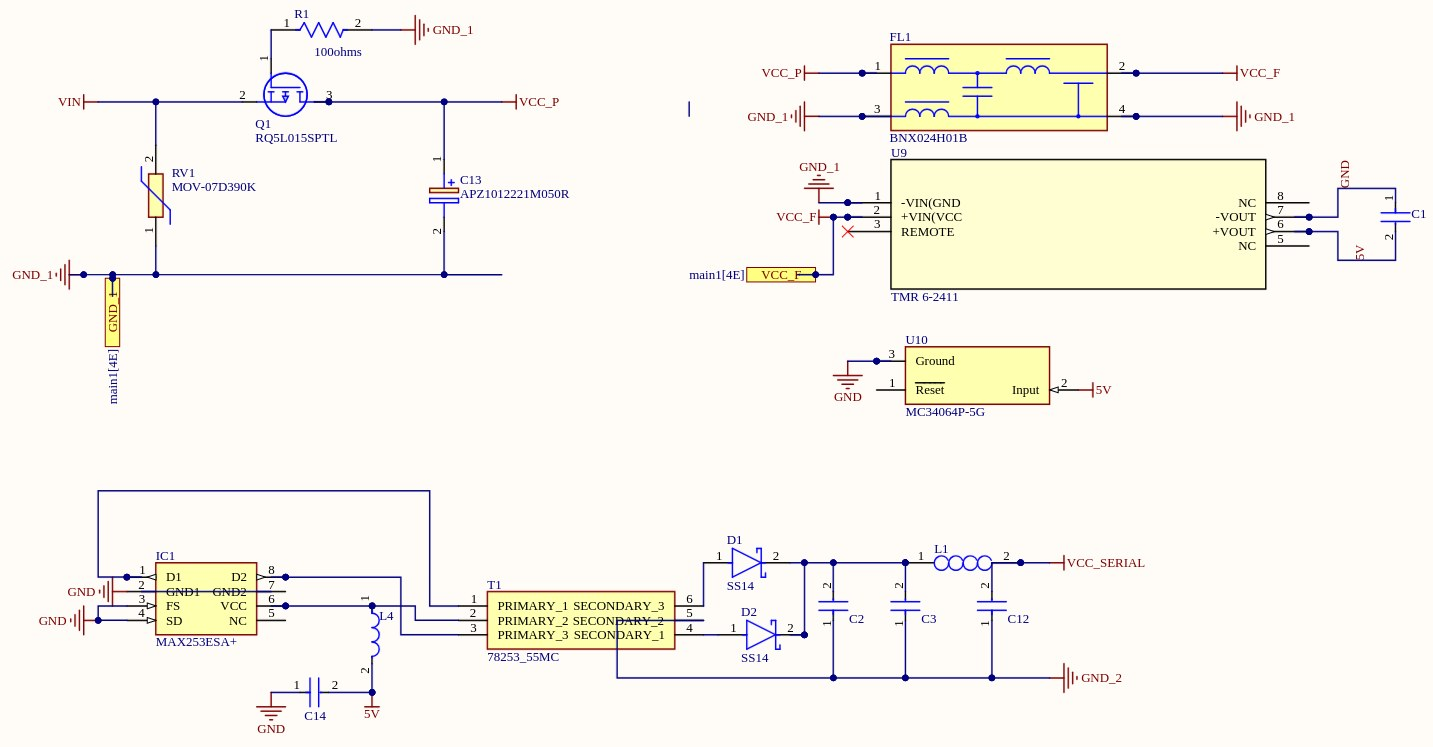
\includegraphics[width=\textwidth]{images/ciclo1_esquematico_mainboard.jpg}
    \fonte{Autoria Própria (Macroentrega V do ciclo I)}
\end{figure}

Na placa de sensores e comunicação, o processador ESP32-S3-Zero recebe os dados do KERNEL e os transmite pelos transceptores RS-422 (ADM489) e RS-232 (MAX3232); o isolador digital ADuM3301 consta como não montado na lista de componentes. A fonte isolada, sem regulação, chegava a 6--10~V em circuitos integrados de 5,5~V. A Figura~\ref{fig:layout_ciclo1} apresenta o \textit{layout} das placas.

\begin{figure}[H]
    \centering
    \caption{\textit{Layout} das placas da fase anterior}
    \label{fig:layout_ciclo1}
    \begin{minipage}[t]{0.32\textwidth}
        \centering
        (a)\\[2pt]
        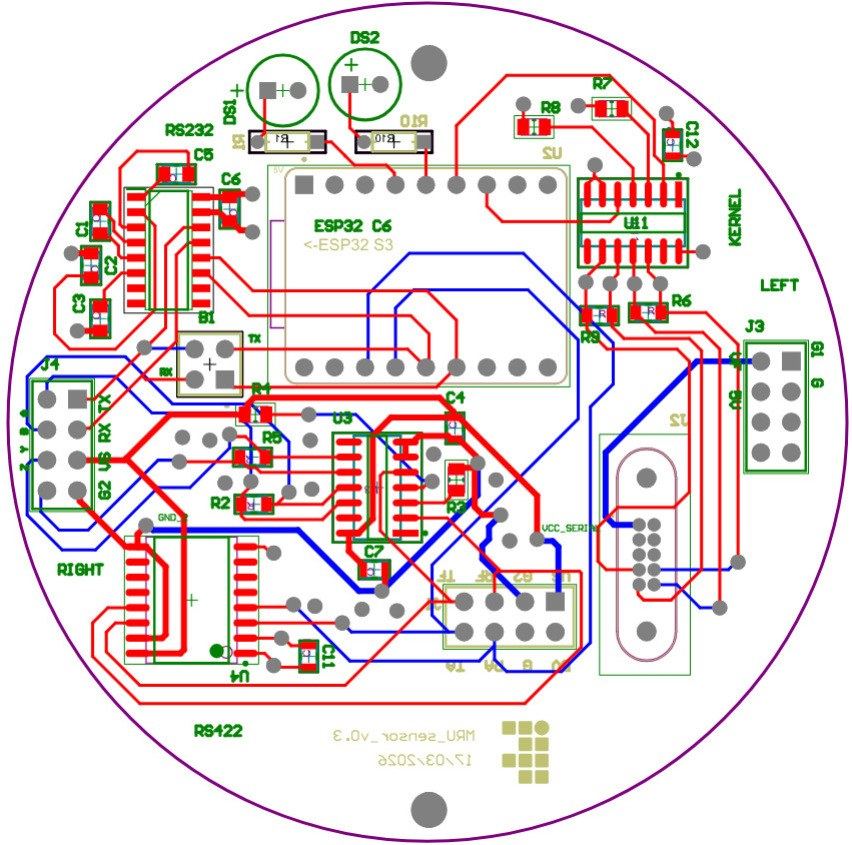
\includegraphics[width=\linewidth]{images/ciclo1_layout_desenho.jpg}
    \end{minipage}\hfill
    \begin{minipage}[t]{0.32\textwidth}
        \centering
        (b)\\[2pt]
        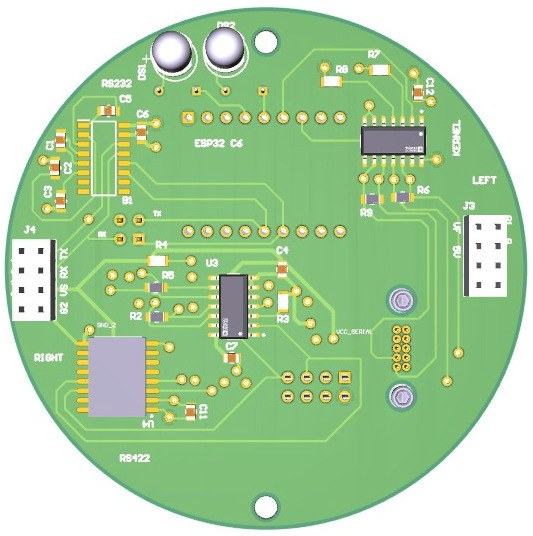
\includegraphics[width=\linewidth]{images/ciclo1_layout_inferior.jpg}
    \end{minipage}\hfill
    \begin{minipage}[t]{0.32\textwidth}
        \centering
        (c)\\[2pt]
        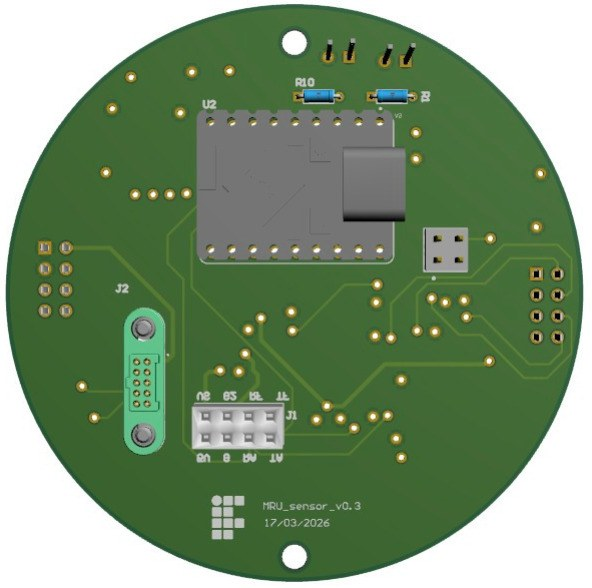
\includegraphics[width=\linewidth]{images/ciclo1_layout_superior.jpg}
    \end{minipage}
    \fonte{Autoria Própria (Macroentrega V do ciclo I). (a) placa modificada (desenho); (b) placa inferior; (c) placa superior}
\end{figure}

\subsubsection{Agora: Placas Revisadas}

% PENDENTE: texto, esquemático e layout das placas revisadas (aguardando a Letícia)
\pendente{[Texto pendente: aguardando as informações das placas revisadas.]}

\begin{figure}[H]
    \centering
    \caption{Esquemático revisado com isolamento galvânico}
    \label{fig:esquematico}
    % PENDENTE: esquemático revisado (Letícia)
    \reservado{5cm}{(inserir esquemático)}
    \fonte{Autoria Própria}
\end{figure}

\begin{figure}[H]
    \centering
    \caption{\textit{Layout} da placa de circuito impresso}
    \label{fig:layout}
    % PENDENTE: layout revisado (Letícia)
    \reservado{5cm}{(inserir \textit{layout} da PCB)}
    \fonte{Autoria Própria}
\end{figure}

\newpage
\section{Atividades Complementares}\label{sec:complementares}

Nesta seção, são apresentadas as atividades complementares realizadas no período: o comparativo entre a NORMAM-27 e a NORMAM-223, o comparativo entre o MRU 5 e o KERNEL-120, a cadeia de processamento e calibração e as posições de montagem, a comunicação e os comandos do equipamento.

\subsection{Comparativo entre a NORMAM-27 e a NORMAM-223}
\label{sec:normam}

A NORMAM-27/DPC, cuja portaria de aprovação foi revogada, foi sucedida pela NORMAM-223/DPC.
Ambas estabelecem os limites de movimento do helideque para operação de aeronaves e os
requisitos do sistema que os monitora (HMS). As grandezas envolvidas são o balanço (B,
\textit{roll}), o caturro (C, \textit{pitch}), a inclinação (Inc), a arfagem (Arf,
\textit{heave}), a velocidade de arfagem (VArf, \textit{heave rate}) e, apenas na
NORMAM-223, a velocidade significativa de arfagem (SVArf), obtida a partir das três maiores
velocidades de arfagem registradas em 20~min ou como duas vezes o seu valor RMS.

A Tabela~\ref{tab:normam} compara os requisitos de aprovação das duas normas.

\begin{small}
\renewcommand{\arraystretch}{1.3}
\begin{longtable}{|m{3.2cm}|m{5.5cm}|m{5.5cm}|}
\caption{Comparativo entre a NORMAM-27 e a NORMAM-223}
\label{tab:normam}\\
\hline
\centering Item & \centering NORMAM-27/DPC Rev.~2 Mod.~4 &
\centering NORMAM-223/DPC Rev.~1 Mod.~1 \tabularnewline \hline
\endfirsthead
\hline
\centering Item & \centering NORMAM-27/DPC Rev.~2 Mod.~4 &
\centering NORMAM-223/DPC Rev.~1 Mod.~1 \tabularnewline \hline
\endhead
Balanço e caturro (B e C) & $\pm1^\circ$ a $\pm4^\circ$, conforme categoria, período e
classe; em boia, $\pm1^\circ$ à noite & $\pm2^\circ$ a $\pm4^\circ$ nas operações
permitidas; em boia, $\pm1^\circ$ à noite \\ \hline
Inclinação (Inc) & 1,5$^\circ$ a 4,5$^\circ$; se não medida, calculada a partir de B e C
pela tabela da norma & 2,5$^\circ$ a 4,5$^\circ$; se não medida, calculada a partir de B e
C pela mesma tabela \\ \hline
Velocidade de arfagem (VArf) & 0,5 a 1,3~m/s & 0,5 a 1,3~m/s \\ \hline
Velocidade significativa de arfagem (SVArf) & Não se aplica & 0,5 a 1,3~m/s (três maiores
velocidades em 20~min, ou 2~$\times$~RMS) \\ \hline
Arfagem (\textit{heave}) & 1,5 a 5,0~m; usada como limite apenas na ausência de VArf &
1,5 a 5,0~m; usada como limite apenas na ausência de VArf e de SVArf \\ \hline
Janela de avaliação & Máximo de 20~min & Máximo de 20~min \\ \hline
Exatidão do sensor & Sem valor numérico; exige dados fidedignos e de precisão adequada &
Sem valor numérico; exige dados fidedignos e de precisão adequada \\ \hline
Movimento em tempo real & Exibido pelo HMS; sem taxa mínima para o sensor & Exibido pelo
HMS; sem taxa mínima para o sensor \\ \hline
Ponto de medição & Sensor no piso do helideque ou valores corrigidos para a altura e a
posição do helideque & Sensor no piso do helideque ou valores corrigidos para a altura e a
posição do helideque \\ \hline
Operação noturna na Classe 3 & Permitida, com B e C de $\pm1^\circ$ (Categoria A) e
$\pm1{,}5^\circ$ (Categoria B) & Vedada; há regra de reclassificação conforme a direção do
vento (§~9.4) \\ \hline
Calibração & Conforme o fabricante ou, sem intervalo definido, a cada 24 meses, segundo
parâmetros da RBC/INMETRO & Conforme o fabricante ou, sem intervalo definido, a cada 24
meses, segundo parâmetros da RBC/INMETRO \\ \hline
Grandezas monitoradas & B, C, Inc, VArf e Arf & B, C, Inc, VArf, SVArf e Arf \\ \hline
Ato normativo & Portaria nº 77 (revogada) & Portaria nº 184 \\ \hline
\end{longtable}
\end{small}
\vspace{-0.6cm}
\fonte{Elaborado a partir da NORMAM-27/DPC Rev.~2 Mod.~4 (Portaria nº 77) e da NORMAM-223/DPC
Rev.~1 Mod.~1 (Portaria nº 184), conforme a triagem de sensores frente às normas de helideque}

Para o sensor, a principal consequência da NORMAM-223 é o cálculo da SVArf, que nenhum dos
sensores avaliados na triagem fornece de forma nativa e que, portanto, fica a cargo do
firmware ou do HMS. As demais exigências sobre o equipamento são idênticas, e a triagem
chegou à mesma conclusão para cada sensor nas duas normas
(Seção~\ref{sec:comparativo}).

\subsection{Comparativo entre o MRU 5 e o KERNEL-120}\label{sec:comparativo}

A Tabela~\ref{tab:comparativo} compara o MRU 5, da Kongsberg, e o KERNEL-120, da Inertial Labs, frente aos requisitos da NORMAM-27 e da NORMAM-223 (Seção~\ref{sec:normam}), conforme a triagem de sensores feita a partir dos \textit{datasheets}. Como as normas não fixam exatidão numérica para o sensor, a triagem verifica se cada grandeza é fornecida pelo equipamento e se está documentada.

{\footnotesize
\renewcommand{\arraystretch}{1.25}
\begin{longtable}{|>{\raggedright\arraybackslash}p{2.2cm}|>{\raggedright\arraybackslash}p{2.4cm}|>{\raggedright\arraybackslash}p{2.4cm}|>{\raggedright\arraybackslash}p{3.2cm}|>{\raggedright\arraybackslash}p{3.0cm}|}
    \caption{Comparativo MRU 5 e KERNEL-120 (NORMAM-27 e NORMAM-223)}\label{tab:comparativo}\\
    \hline
    \centering\arraybackslash\textbf{Requisito} & \centering\arraybackslash\textbf{NORMAM-27} & \centering\arraybackslash\textbf{NORMAM-223} & \centering\arraybackslash\textbf{MRU 5} & \centering\arraybackslash\textbf{KERNEL-120} \\ \hline
    \endfirsthead
    \hline
    \centering\arraybackslash\textbf{Requisito} & \centering\arraybackslash\textbf{NORMAM-27} & \centering\arraybackslash\textbf{NORMAM-223} & \centering\arraybackslash\textbf{MRU 5} & \centering\arraybackslash\textbf{KERNEL-120} \\ \hline
    \endhead
    \multicolumn{5}{r}{\textit{continua na próxima página}} \\
    \endfoot
    \endlastfoot
    Balanço e caturro (B e C) & $\pm1^\circ$ a $\pm4^\circ$ & $\pm2^\circ$ a $\pm4^\circ$ & 0,02$^\circ$ RMS estático; 0,005$^\circ$ (1$\sigma$) dinâmico & 0,05$^\circ$ RMS estático; 0,08$^\circ$ RMS dinâmico \\ \hline
    Inclinação (Inc) & 1,5$^\circ$ a 4,5$^\circ$ & 2,5$^\circ$ a 4,5$^\circ$ & Pode ser derivada de B e C no HMS & Pode ser derivada de B e C no HMS \\ \hline
    Velocidade de arfagem (VArf) & 0,5 a 1,3~m/s & 0,5 a 1,3~m/s & Saída nativa; 0,01~m/s RMS & Não consta nas saídas \\ \hline
    SVArf & Não se aplica & 0,5 a 1,3~m/s & Sem saída nativa; cálculo pelo HMS & Sem saída nativa; depende de algoritmo do HMS \\ \hline
    Arfagem (Arf) & 1,5 a 5,0~m, só sem VArf & 1,5 a 5,0~m, só sem VArf e SVArf & Saída nativa; 5~cm ou 5\,\% em tempo real e 1~cm ou 1\,\% na saída retardada & Não consta nas saídas \\ \hline
    Taxa de saída & Sem mínimo para o sensor & Sem mínimo para o sensor & Até 200~Hz & Até 2000~Hz (IMU e B/C) \\ \hline
    Ponto de medição & Piso do helideque ou valores corrigidos & Piso do helideque ou valores corrigidos & CG e dois pontos configuráveis & Correção não declarada \\ \hline
    Qualidade dos dados & Dados fidedignos & Dados fidedignos & Palavra de \textit{status} & BIT contínuo \\ \hline
    Calibração & Fabricante ou 24 meses (RBC) & Fabricante ou 24 meses (RBC) & Certificado individual de fábrica & Calibrado em temperatura; RBC não demonstrada \\ \hline
    \textbf{Conclusão} & \multicolumn{2}{c|}{Igual nas duas normas} & \textbf{Aprovado} & \textbf{Aprovado com ressalvas} \\ \hline
\end{longtable}
}
{\vspace{-0.5\baselineskip}\fonte{Elaborado a partir da triagem de sensores frente às normas de helideque (NORMAM-27 Rev.~2 Mod.~4 e NORMAM-223 Rev.~1 Mod.~1) e dos \textit{datasheets} do MRU 5 (Kongsberg, rev.~E, 2025) e do KERNEL-120 (Inertial Labs)}\par}

Em balanço e caturro, os dois sensores fornecem a grandeza pronta, e o MRU 5 tem exatidão melhor. A diferença decisiva está na arfagem e na velocidade de arfagem: o MRU 5 as fornece de forma nativa e com exatidão declarada, enquanto o KERNEL-120 não as fornece. No DRMM, o \textit{firmware} calcula o \textit{heave} a partir da aceleração vertical e o leva até o centro do helideque pelo braço de alavanca, enviando ao HMS o \textit{heave} e o \textit{heave rate} (Seção~\ref{sec:pipeline}). É esse cálculo que precisa ser validado em ensaio para que a ressalva seja retirada. Nos dois casos, a aprovação final depende da integração com o HMS, de ensaio e de calibração da instalação.

\subsection{Cadeia de Processamento e Calibração}\label{sec:pipeline}

A Figura~\ref{fig:pipeline} (Seção~\ref{sec:metodologia}) resume a cadeia de processamento do Measure MRU, conforme o \href{\urldatasheet}{\textit{datasheet} do equipamento}. Cada uma das cinco etapas tem uma parte ajustada uma vez por unidade, no ensaio contra a mesa de referência (calibração \textit{offline}), e uma parte executada pelo \textit{firmware} a cada amostra, com os parâmetros gravados nesse ensaio, na posição de montagem de bordo.

No filtro, a calibração escolhe, para cada eixo, o filtro e a frequência de corte com o menor erro $\varepsilon$ de Wiener, e o \textit{firmware} aplica um pré-filtro passa-baixa por eixo na taxa de aquisição. Na correção, o ensaio estima o alinhamento de montagem (problema de Wahba) e os coeficientes $M$, $c$ e $k$ por regressão \textit{ridge}, e o \textit{firmware} aplica $x = M x + c + k\,\Delta T$, levando as medidas aos eixos do navio e removendo os erros de escala, de alinhamento e de temperatura. Na atitude, a calibração compara o filtro de Kalman, o ajuste linear e o aprendizado de máquina e exporta o escolhido, e o \textit{firmware} calcula \textit{roll}, \textit{pitch} e \textit{yaw} com um filtro de Kalman de estado de erro (ESKF) de 6 estados, com integração \textit{strapdown} e compensação de \textit{coning}. No \textit{heave}, os parâmetros são escolhidos em uma grade de período $T_h$ e amortecimento $\zeta$, e o \textit{firmware} obtém o \textit{heave} no sensor a partir da aceleração vertical, por dupla integração com filtro passa-alta. No braço, informa-se a posição do helideque em relação ao MRU, e o \textit{firmware} translada o movimento até esse ponto, fornecendo $h$ e $h_r$ no centro do helideque.

Ao final do ensaio, o RMS contra a referência é calculado para a inclinação, o \textit{heave} e o \textit{heave rate}, e o certificado registra, por eixo, se cada requisito foi atendido. A bordo, uma janela móvel de 20~min, atualizada a cada 1~s, calcula as grandezas da NORMAM (B, C, Inc, Arf, VArf e SVArf), e a saída é enviada nos modos CALIBRATED, RAW ou SCALE, em JSON, LIST ou NMEA.

\subsection{Posições de Montagem, Comunicação e Comandos}
\label{sec:montagem}

O MRU pode ser instalado em quatro posições. O comando \texttt{\$align:N!} grava a
orientação de montagem, e ângulos, acelerações e velocidades angulares passam a ser
fornecidos nos eixos do navio. A Tabela~\ref{tab:montagem} relaciona cada posição ao
comando correspondente e aos ângulos gravados.

\begin{table}[H]
\centering
\caption{Posições de montagem e comandos de alinhamento}
\label{tab:montagem}
\small
\renewcommand{\arraystretch}{1.3}
\begin{tabularx}{\textwidth}{|m{3cm}|m{2.4cm}|Y|m{3.6cm}|}
\hline
\centering Posição & \centering Comando & \centering Montagem & \centering Ângulos gravados
(proa, pitch, roll) \tabularnewline \hline
Em pé & \texttt{\$align:1!} & Base no convés, cabo para cima & 0$^\circ$; $-90^\circ$;
0$^\circ$ \\ \hline
Cabeça para baixo & \texttt{\$align:2!} & Base no teto, cabo para baixo & 0$^\circ$;
$+90^\circ$; 0$^\circ$ \\ \hline
Parede à vante & \texttt{\$align:0!} & Base na antepara de vante, cabo para ré &
0$^\circ$; 0$^\circ$; 0$^\circ$ \\ \hline
Parede à ré & \texttt{\$align:4!} & Base na antepara de ré, cabo para vante & 180$^\circ$;
0$^\circ$; 180$^\circ$ \\ \hline
\end{tabularx}
\fonte{Adaptado do \href{\urldatasheet}{datasheet do Measure MRU}}
\end{table}

Na instalação, a marca X do tampo deve apontar sempre para boreste: com a marca voltada
para a proa, pitch e roll trocam de lugar e, voltada para bombordo, trocam de sinal. Após o
comando de alinhamento, o MRU deve ser desligado e religado, pois a orientação é aplicada
ao energizar. A calibração vale para a posição e o alinhamento do ensaio, e uma mudança de
posição exige nova calibração. Montagens no costado ou com a marca na vertical não possuem
posição predefinida.

As portas RS-422, RS-232 e USB aceitam os mesmos comandos em texto ASCII, delimitados por
\texttt{\$} e \texttt{!}, e as configurações ficam gravadas em memória não volátil. O MRU
responde na porta que enviou o último comando, e o fluxo de dados passa a sair por ela. A
Tabela~\ref{tab:comandos} apresenta os comandos de operação disponíveis.

\begin{table}[H]
\centering
\caption{Comandos de operação}
\label{tab:comandos}
\small
\renewcommand{\arraystretch}{1.3}
\begin{tabularx}{\textwidth}{|m{4.5cm}|Y|}
\hline
\centering Comando & \centering Efeito \tabularnewline \hline
\texttt{\$stream\_start!} & Liga o fluxo de dados na porta \\ \hline
\texttt{\$stream\_stop!} & Desliga o fluxo de dados \\ \hline
\texttt{\$settings!} & Retorna as configurações, em JSON \\ \hline
\texttt{\$check\_sensor!} & Retorna OK ou NOT WORKING \\ \hline
\texttt{\$firmware!} & Retorna a versão do firmware \\ \hline
\texttt{\$align:N!} & Grava a posição de montagem (0, 1, 2 ou 4) \\ \hline
\texttt{\$ackoneledge!} & Teste de comunicação \\ \hline
\texttt{\$ERASE!} & Restaura os padrões \\ \hline
\end{tabularx}
\fonte{Adaptado do \href{\urldatasheet}{datasheet do Measure MRU}}
\end{table}

As configurações são gravadas pelo comando \texttt{CF:chave\$valor!} e lidas pelo comando \texttt{ID:chave\$}, com as chaves e os valores apresentados na Tabela~\ref{tab:chaves}.

\begin{table}[H]
\centering
\caption{Configurações gravadas por \texttt{CF:chave\$valor!} e lidas por \texttt{ID:chave\$}}
\label{tab:chaves}
\small
\renewcommand{\arraystretch}{1.3}
\begin{tabularx}{\textwidth}{|m{3.2cm}|Y|m{2cm}|}
\hline
\centering Chave & \centering Valores & \centering Padrão \tabularnewline \hline
\texttt{device\_mode} & 0 NORMAL; 1 ACQUISITION & 0 \\ \hline
\texttt{streamer\_mode} & 0 CALIBRATED; 1 RAW; 2 SCALE & 0 \\ \hline
\texttt{protocol} & 0 JSON; 1 LIST; 2 NMEA & 0 \\ \hline
\texttt{frequency} & Frequência do fluxo, em Hz, até 100 & 100 \\ \hline
\texttt{baudrate} & Taxa de transmissão da RS-232 e da RS-422 & 9600 \\ \hline
\texttt{autostream} & 1 transmite ao ligar & 0 \\ \hline
\end{tabularx}
\fonte{Adaptado do \href{\urldatasheet}{datasheet do Measure MRU}}
\end{table}

Cada comando \texttt{CF:} grava a chave e reinicia o equipamento, de modo que os comandos
devem ser enviados um por vez, aguardando o retorno. Na saída NMEA 0183, o MRU transmite a
sentença \texttt{\$GPPASHR,pitch,roll,yaw,heave*CS}, com ângulos em graus, \textit{heave}
em metros e \textit{checksum} XOR em hexadecimal.



\newpage
\section{Considerações Finais}\label{sec:consideracoes}

Esta macroentrega iniciou a segunda fase do projeto com a preparação do DRMM para atmosferas explosivas. O mapeamento de lacunas confrontou o protótipo da fase anterior com as normas ABNT NBR IEC 60079-0, 60079-1 e 60079-7 e com a Portaria Inmetro nº 115/2022. O invólucro metálico atende ao requisito de eletrostática, e a potência de cerca de 3,6~W cumpre a classe de temperatura T4; as lacunas estão na proteção da entrada de alimentação, nas conexões internas, no módulo processador, na entrada de cabos, no aterramento e na marcação, além das juntas à prova de chama, no caso do Ex d.

A comparação entre os tipos de proteção reduziu as alternativas viáveis a duas: o invólucro à prova de explosão (Ex db), para Zona~1, e a segurança aumentada (Ex ec), para Zona~2, ambas com grupo de gás IIC e classe de temperatura T4. Os MRUs concorrentes não possuem certificação Ex e usam caixas à parte, e um MRU certificado seria um diferencial; a escolha depende da zona do helideque, que deve ser pedida à operadora. O estudo recomenda projetar a placa já pensando no Ex ec, pois ela continua servindo dentro de um invólucro Ex d.

Foram modeladas três alternativas de invólucro, das quais a de parafusos verticais foi a mais bem avaliada pela empresa de usinagem, com o alumínio 6061-T5 considerado como material. O ensaio térmico mostrou que o sensor estabiliza em torno de 64~°C, dentro da faixa de atuação do KERNEL, e a dissipação de temperatura ainda será melhorada. Na eletrônica, foram definidas as alterações de componentes, com destaque para o isolamento galvânico da RS-422 por meio do ADM2587E, que substitui o estágio isolado da fase anterior. As atividades complementares consolidaram os requisitos da NORMAM-27 e da NORMAM-223 para o sensor, a comparação entre o MRU 5 e o KERNEL-120 e a documentação da cadeia de processamento e dos comandos do equipamento.

Como próximos passos, destacam-se a obtenção da classificação de áreas do helideque, a definição do invólucro e a sua simulação mecânica e térmica, a medição das temperaturas com o invólucro e a eletrônica revisados, a conclusão dos esquemáticos e do \textit{layout} e a confirmação de pontos com o Organismo de Certificação de Produto (OCP). A Macroentrega 2 prevê a homologação de fornecedores, a aquisição de insumos e a usinagem dos invólucros.

% ===============================================================
\newpage
\bibliography{references}
\end{document}
